\documentclass[12pt]{article}
\usepackage[english]{babel}
\usepackage[left=1in,top=1in,right=1in,bottom=1in]{geometry}
\usepackage{tabularx}
\usepackage{amsmath, amssymb, amsthm}
\usepackage{graphicx}
\usepackage{caption}
\usepackage{enumitem}
\usepackage{pgfplots}
\usepackage{accents}
\usepackage{natbib}
\usepackage{float}
\usepackage[bottom, flushmargin]{footmisc}
\usepackage{bm}
\usepackage{lipsum}
\usepackage{changepage}
\usepackage{dsfont}
\usepackage{multirow}
\usepackage{setspace}
\usepackage{threeparttable}
\usepackage{booktabs}

% Set directories
\graphicspath{{../output/figures/}}
\newcommand{\inputpath}{../output/tables/}

% Font
\usepackage{palatino} 

% Colors
\definecolor{beamerblue}{rgb}{0.2,0.2,0.7}
\definecolor{dgreen}{rgb}{0,0.55,0}
\definecolor{winered}{rgb}{0.5,0,0}

% Bibliography style
\bibliographystyle{chicago}
\setcitestyle{authoryear,open={(},close={)}}
\usepackage[colorlinks=true, allcolors=beamerblue,urlcolor=beamerblue]{hyperref}

% For defining theorems
\newtheorem{theorem}{Theorem}[section]
\newtheorem{definition}{Definition}[section]
\newtheorem{corollary}{Corollary}[theorem]
\newtheorem{lemma}[theorem]{Lemma}
\newtheorem{assumption}{Assumption}

% Figures/graphics
\usepackage{morefloats}
\usepackage{graphicx}
\usepackage{caption}
\usepackage{subcaption}

% Math symbols
\DeclareMathOperator*{\argmax}{arg\,max}
\DeclareMathOperator*{\argmin}{arg\,min}
\def\mathbi#1{\textbf{\em #1}}
\DeclareMathOperator{\vect}{vec}
\newcommand{\Var}{\mathrm{Var}}
\newcommand{\Cov}{\mathrm{Cov}}
\newcommand{\ubar}[1]{\underaccent{\bar}{#1}}

% Spacing 
\setlength{\parindent}{0.75cm}	% Paragraph Indentation
\setstretch{1.5} 				% Line Space

% Title and author information
\title{The Ins and Outs of Unemployment Shocks\thanks{This paper is a heavily revised version of the third chapter of my PhD dissertation at Boston College. I thank Theodore Papageorgiou, Robert Ulbricht, and Hanno Foerster for their invaluable guidance and support. I am also grateful to Hie Joo Ahn, Ben Bridgman, Gary Cornwall, Cynthia Doniger, and seminar participants at Salisbury University, MEA 2024, and SEA 2024 for helpful discussions and suggestions. Declarations of interest: none. The views expressed in this paper are solely those of the author and not necessarily those of the U.S. Bureau of Economic Analysis (BEA) or the U.S. Department of Commerce. Research initiated prior to the author's employment at BEA.}} 
\author{Carter Bryson\thanks{Email: carter.bryson@bea.gov. Address: U.S. Department of Commerce, Bureau of Economic Analysis, 4600 Silver Hill Road, Suitland, MD 20746}}
\date{\today}

% Start of document
\begin{document}
\maketitle
\thispagestyle{empty}

%%%%%%%%%%%%%%%%%%%%%%%%%%%%%%%%%%%%%%%%%%%%%%
% Abstract %%%%%%%%%%%%%%%%%%%%%%%%%%%%%%%%%%%%%%%%
%%%%%%%%%%%%%%%%%%%%%%%%%%%%%%%%%%%%%%%%%%%%%%
\begin{abstract}
This paper quantifies the roles of unemployment inflows and outflows in cyclical unemployment. Motivated by the joint dynamic relationship between worker flows and the unemployment rate, I design a simple identification strategy that accounts for this pattern and use it to empirically isolate changes in job separation and job finding. I find that both margins contribute significantly to unemployment volatility and that their interaction is important for understanding the business-cycle dynamics of the unemployment rate. In particular, an initial spike in job loss leads to a future decline in the job finding rate, supporting mechanisms from a newer class of models that predict this behavior. My results caution against ignoring cyclical variation in job loss and suggest that macroeconomic models of the labor market should aim to explicitly capture the dynamic interaction between the ins and outs of unemployment.
\vfill\noindent
\textbf{Keywords:} Worker Flows, Unemployment, Business Cycles, Sign Restrictions \\
\textbf{JEL Classification:} C32, E24, E32, J64
\end{abstract}

%%%%%%%%%%%%%%%%%%%%%%%%%%%%%%%%%%%%%%%%%%%%%%
% Introduction %%%%%%%%%%%%%%%%%%%%%%%%%%%%%%%%%%%%%%
%%%%%%%%%%%%%%%%%%%%%%%%%%%%%%%%%%%%%%%%%%%%%%
\clearpage
\pagenumbering{arabic} 

\section{Introduction}\label{sec:intro}

What accounts for the rise in the unemployment rate during a recession? Economists have debated this seemingly straightforward question going back at least five decades \citep{Darby:1986aa, Blanchard:1990aa, Elsby:2009aa, Shimer:2012aa, Mercan:2024aa}. Reaching a definitive conclusion has proved challenging because it requires quantifying the contributions of two different, but interlinked channels: in recessions, employed workers lose jobs, but unemployed workers also have trouble finding jobs. Previous studies have typically used simple accounting decompositions motivated by search and matching theory to separately assess the roles of unemployment inflows and outflows, often yielding conflicting results.

In this paper, I provide new empirical evidence on how inflows to and outflows from unemployment contribute to the business-cycle dynamics of the labor market. Rather than using a simple decomposition framework, I treat unemployment and worker flows as part of a jointly determined system and implement an empirical identification strategy to recover shocks to inflow and outflow rates. This allows me to assess the contribution of each margin while accounting for its \textit{dynamic} effects on other labor market variables. I find that unemployment inflows play a large role in unemployment fluctuations not only because they result in contemporaneous changes in the pool of unemployed workers but also because they lead to \textit{future} movements in unemployment outflows.

To motivate my analysis, I first examine the dynamic properties of unemployment inflows and outflows and present three pieces of evidence. First, while the \textit{rate} at which workers find jobs out of unemployment is procyclical, the \textit{number} of workers that find jobs out of unemployment is countercyclical. Somewhat surprisingly, this indicates that more unemployed workers find jobs in recessions than in expansions, but they account for a lower proportion of total unemployment. Next, aggregate unemployment outflows (job finding) are, on average, predated by aggregate unemployment inflows (job separation).\footnote{I use the term ``job separation'' to refer to movements of workers from employment to unemployment ($EU$ flows). Of course, true job separations include instances where a worker moves from employment to not-in-the-labor-force ($EN$ flows) or from one employer to another (employer-to-employer flows). However, labeling $EU$ flows as ``job separation'' and $UE$ flows as ``job finding'' provides a convenient shorthand. See Section \ref{sec:data} for more details on terminology.} I find that both the job finding rate and the unemployment rate display the strongest cross-correlations with lagged rather than contemporaneous values of the job separation rate. Last, I test formally for Granger causality and find that unemployment inflows Granger-cause unemployment outflows. Hence, the relationship between the stock of unemployment and the flows into and out of unemployment is characterized by a specific dynamic structure. While this evidence is not entirely new to the literature, it forms the basis of my empirical identification strategy.\footnote{\cite{Fujita:2009aa} and \cite{Barnichon:2012aa} also document the lead-lag structure of job separation and job finding and emphasize the importance of dynamic interactions between these variables in accounting for unemployment fluctuations. Though similar in spirit to these papers, my approach allows me to directly estimate how innovations to inflows and outflows affect the labor market while remaining agnostic to the specific set of underlying structural shocks.}

Then, I specify a structural vector autoregression (SVAR) model and implement a simple identification strategy motivated by this evidence in order to isolate disturbances in the variables that govern unemployment dynamics. The goal is to estimate how job finding, job separation, the unemployment rate, and average unemployment duration respond to exogenous changes in these variables and to decompose their fluctuations over the business cycle. This approach allows me to formally examine the roles played by changes in unemployment inflows and outflows in driving the unemployment rate, utilizing several techniques familiar to the SVAR literature.

A benefit of this approach is that it does not require that certain worker flow margins be held constant when examining the contribution of others \citep{Shimer:2012aa}. For instance, a spike in job separations may feed back on job creation incentives, in turn affecting the job finding rate. In this case, my methodology accounts for the endogenous reaction of the job finding rate to an initial impulse in unemployment inflows. Although the procedure I use does not identify the underlying fundamental disturbances that drive business cycles, the properties of the unemployment inflow and outflow ``shocks'' that I recover shed light on the forces that contribute to the cyclical variance of unemployment.

The assumptions behind my identification strategy rest on the time series properties of worker flows I document as well as the relationship between worker flows and the distribution of unemployment duration. The evidence on the lead-lag structure of worker flows implies that job separations do not react immediately to changes in job finding or unemployment. I therefore restrict the impact response of the unemployment rate and the job finding rate to be zero following a shock to job separation. I supplement these zero restrictions with sign restrictions on the response of the unemployment rate and average unemployment duration to innovations in job finding and job separation. I assume that while shocks to job finding move the unemployment rate and average unemployment duration in the same direction, shocks to job separation move the unemployment rate and average unemployment duration in opposite directions.\footnote{The logic for these assumptions is as follows: all else equal, an increase in the frequency of unemployment inflows leads to a rise in the unemployment rate and a fall in average unemployment duration, as newly unemployed workers have 0 unemployment duration by construction. Conversely, all else equal, a decrease in the frequency of unemployment outflows leads to a rise in the unemployment rate and a rise in average unemployment duration, as it increases expected unemployment duration.} Finally, I assume innovations in the unemployment rate negatively impact average unemployment duration, all else equal, imposing additional discipline on the forces that change the level and duration of unemployment simultaneously.\footnote{I think of shocks to the unemployment rate, holding the job finding and job separation rates constant, as capturing movements into the unemployed pool from outside the labor force, in which case unemployment duration is also 0 by construction. I thank an anonymous referee for this suggestion.}

Because my identification strategy combines both zero and sign restrictions, I use Bayesian techniques to estimate the model following recent advances in the literature \citep{Rubio:2010aa, Arias:2018aa}. My baseline specification includes four variables: the job finding probability, the job separation probability, the unemployment rate, and average unemployment duration for the period 1948Q1--2019Q4.\footnote{I exclude the most recent recession induced by the COVID pandemic because of its stark and unusual labor market dynamics. However, I confirm in the Appendix that my baseline results remain unchanged after including 2020Q1--2024Q4 in my sample.} I recover four shocks in total, which I label as shocks to the Unemployment Inflow, Unemployment Outflow, Unemployment Level, and Unemployment Length.

I find that Unemployment Inflow shocks lead to large movements in all four series. In response to a (contractionary) Unemployment Inflow shock, the job separation probability increases significantly and remains elevated for almost two years. The job finding probability reacts little on impact, but then falls for several periods before slowly returning to trend. The unemployment rate rises on impact and displays a hump-shaped pattern: the initial increase in job separation increases unemployment and the subsequent decline in job finding causes it to rise further. Lastly, average unemployment duration falls on impact, but then follows an increasing, hump-shaped pattern as workers accumulate in the unemployment pool. In contrast, while (contractionary) Unemployment Outflow shocks lead to increases in the unemployment rate and average unemployment duration, they are of smaller magnitude and are not associated with increases in the job separation probability. Moreover, I do not find that Unemployment Level or Length shocks lead to large, significant deviations in either the job separation or job finding probability.
 
Next, I use local projections to assess the impact of unemployment inflow and outflow shocks on auxiliary labor market variables \citep{Jorda:2005aa}. I find that while unemployment inflow shocks are consistent with the business-cycle properties of gross worker flows and vacancy posting, unemployment outflow shocks are not. In particular, a contractionary unemployment inflow shock leads to an increase in the \textit{total} flow of workers between unemployment-and-employment and between employment-and-unemployment. Because both of these series are countercyclical in the data, changes in unemployment inflows are plausible drivers of gross worker flows over the business cycle. Additionally, unemployment inflow shocks lead to large changes in vacancy posting. I find that the level of vacancies falls by about 6\% following a contractionary inflow shock. This pattern is consistent with Beveridge Curve dynamics, as unemployment and vacancies move in opposite directions. On the other hand, unemployment outflow shocks do not lead to significant movements in gross worker flows or vacancies.\footnote{I view these results as a contribution of my approach relative to previous studies that either directly estimate or impose restrictions on the behavior of vacancies or market tightness \citep{Fujita:2011aa, Mercan:2024aa}. However, I show in the appendix that my results are robust to including vacancies in the VAR.}

Having documented the properties of unemployment inflow and outflow shocks, I turn to quantifying their contributions to fluctuations in unemployment. I find that on average, unemployment inflow shocks explain about 45\% of the overall variance of the unemployment rate, while unemployment outflow shocks account for only about 15\%.\footnote{Note that this implies the inflow margin is 3 times more important than the outflow margin, in direct contrast to the results in \cite{Shimer:2012aa} where it is only 1/3 as important.} However, I note several caveats to this result. First, their contributions are not constant across horizons; unemployment outflow shocks display larger contributions at shorter horizons. Second, the \textit{interaction} between job finding and job separation in response to unemployment inflow shocks greatly affects this calculation. I find that shutting down their interaction such that the job separation probability does not endogenously affect the job finding probability (and vice versa) significantly decreases (increases) the contribution of unemployment inflow (outflow) shocks to unemployment variance. Lastly, the mix of unemployment inflow and outflow shocks has been different in different recessions. While unemployment inflow shocks primarily drove the persistent rise in unemployment during the 2008 recession, unemployment outflow shocks played a greater role in labor market dynamics during the 2001 recession. This suggests that to understand the cyclical behavior of the unemployment rate, both margins should be considered in conjunction.

Though I find limited responses to unemployment level and unemployment length shocks on average, I do find that they play a significant role in labor market dynamics, particularly in specific recessions. Unemployment level shocks, which capture changes in the relative size of the unemployment pool driven by movements into and out of the labor force, help explain the persistently high unemployment rate after the Great Recession. Likewise, unemployment length shocks, which capture compositional shifts in the pool of unemployed workers, help account for elevated unemployment at longer durations into the recovery. These results further underscore the importance of analyzing different margins of labor market flows in conjunction.

I conclude by discussing the implications of my findings for the development of macroeconomic models of the labor market. Since the influential work of \cite{Shimer:2005aa,Shimer:2012aa}, much of the literature's focus shifted toward modeling forces that generate cyclical movements in the job finding rate, while treating the job separation rate as exogenous and acyclical. Though I am not the first to point this out, the dynamic relationship between unemployment inflows and outflows cautions against this approach.\footnote{In particular, see discussions in \cite{Elsby:2009aa}, \cite{Fujita:2009aa}, \cite{Fujita:2011aa}, \cite{Fujita:2012aa}, and \cite{Mercan:2024aa}, among others.} In addition to not being able to explain the increase in gross unemployment outflows during a recession, treating the job separation probability as fixed does not allow for a connection between changes in inflows and outflows by assumption. My results suggest not only that future research should seek to understand the forces responsible for cyclical variation in job loss, but also that the interaction between unemployment inflows and outflows is a key feature of labor market fluctuations that macroeconomic models should explicitly capture. 

% Literature %%%%%%%%%%%%%%%
\paragraph{Related literature} My paper contributes to a large, longstanding literature studying the dynamics of labor market flows. In a seminal paper, \cite{Darby:1986aa} find that the flow into unemployment is the main determinant of the unemployment rate and declare that ``the ins win.'' \cite{Blanchard:1990aa} show that the amplitude of changes in the total inflow to unemployment is larger than the amplitude of changes in the total outflow, and conclude that reduced employment in a recession results from higher job destruction. \cite{Hall:2005aa} and \cite{Shimer:2012aa} instead argue that contrary to the conventional wisdom, most of the recessionary increase in unemployment results from a fall in the job finding probability.\footnote{Related to this argument, several papers have assessed the ability of the \cite{Mortensen:1994aa} model to account for fluctuations in labor market variables. See, for instance, \cite{Mortensen:2007aa}, \cite{Mortensen:2008aa}, \cite{Pissarides:2009aa}, \cite{Fujita:2012aa}, and \cite{Tortorice:2013aa}.} In my study, I attempt to reconcile the evidence in both sets of papers by examining the behavior of the \textit{total number} of workers exiting or entering unemployment as well as the \textit{probability} of unemployment inflows and outflows.

My results suggest that considering movements in the job finding rate alone paints an incomplete picture of labor market fluctuations, in line with several previous studies. \cite{Elsby:2009aa} argue that it is important to understand both procyclical changes in the job finding rate and countercyclical changes in the job separation rate. \cite{Fujita:2009aa} find that allowing for a dynamic interaction between job finding and job separation leads to a larger contribution of the separation rate. \cite{Fujita:2011aa} uses sign restrictions on the joint behavior of unemployment and vacancies and finds that the dynamics of job loss help explain the cyclical behavior of labor market variables. \cite{Demiralp:2011aa} find evidence of multicointegration among the stock of unemployment and the flows into and out of unemployment. \cite{Canova:2013aa} find that the impact response of unemployment to macroeconomic shocks is primarily driven by the job separation rate, while the job finding rate accounts for most of its persistence. As in these papers, my findings support the interpretation that unemployment initially increases in a recession due to a wave of layoffs and remains high due to a slow recovery in the job finding rate. 

My paper estimates that the job finding probability declines after an initial increase in unemployment inflows, providing empirical support for various theoretical mechanisms outlined in recent studies. For instance, \cite{Ahn:2020aa} and \cite{Gregory:2025aa} argue that if workers with lower intrinsic job finding rates disproportionately enter unemployment in recessions, then this compositional change in the unemployment pool negatively affects the aggregate job finding rate. \cite{Coles:2018aa} show that if vacancy creation is less than infinitely elastic, as is typically assumed in standard search-and-matching models, then job separation shocks play a substantial role in unemployment fluctuations. \cite{Mercan:2024aa} argue that increases in the separation rate reduce job creation incentives because ``congestion'' in hiring decisions renders firms unable to fully absorb the resulting increase in unemployment. Importantly, I find that the propagation of current job separations to future job finding is a robust feature of the data, one that models with endogenous separations do not necessarily capture without incorporating one of the mechanisms discussed above.\footnote{I thank an anonymous referee for encouraging me to highlight this finding.}

Lastly, my paper contributes to the literature on SVAR identification using a combination of zero and sign restrictions. In a seminal paper, \cite{Rubio:2010aa} provide general conditions for identification in SVAR models and develop efficient algorithms for estimation and inference. \cite{Arias:2018aa} build on the methodology in \cite{Rubio:2010aa} and extend their results to allow for both sign and zero restrictions. \cite{Arias:2019aa} apply this methodology in order to identify the effects of monetary policy shocks on output and prices. Though I make no theoretical contributions of my own, my study is the first to my knowledge to apply this methodology in the context of the literature on the ins and outs of unemployment.

% Layout %%%%%%%%%%%%%%%
\paragraph{Layout} The rest of the paper is structured as follows. Section \ref{sec:data} describes how I measure worker flows and Section \ref{sec:motivation} presents motivating evidence for the identifying restrictions used in my empirical analysis. In Section \ref{sec:empirics}, I describe the empirical strategy in detail and discuss the identification assumptions. In Section \ref{sec:results}, I present estimates of the effect of unemployment shocks on different labor market variables and use the results to formally decompose overall fluctuations in unemployment. Section \ref{sec:implications} discusses the implications of my findings for models of the labor market. Section \ref{sec:conclusion} concludes.

%%%%%%%%%%%%%%%%%%%%%%%%%%%%%%%%%%%%%%%%%%%%%%
% Data %%%%%%%%%%%%%%%%%%%%%%%%%%%%%%%%%%%%%%%%%%
%%%%%%%%%%%%%%%%%%%%%%%%%%%%%%%%%%%%%%%%%%%%%%
\section{Measuring Worker Flows}\label{sec:data}

I measure worker transitions across labor market states using microdata from the Current Population Survey (CPS) and publicly available aggregate data from the Bureau of Labor Statistics (BLS). I employ two separate methodologies to measure worker flows, which both follow \cite{Shimer:2012aa}.  This section describes how I construct these measures and also serves to define key terms that I will use throughout the rest of the paper. 

\subsection{Two-State Model}

The first approach constructs the inflow rate to unemployment and the outflow rate from unemployment abstracting from movements into and out of the labor force. I follow \cite{Shimer:2012aa} and define the job finding probability $F_t$ for some interval $[t,t+1)$ as:
\begin{equation}\label{eqn:Ft}
F_t = 1 - \frac{U_{t+1} - U^s_{t+1}}{U_t}
\end{equation}
where $U_t$ is total unemployment and $U^s_t$ is total short-term unemployment in month $t$. Both series are published by the BLS starting in January 1948.\footnote{Specifically, I directly download the series LNS13000000: Unemployment Level and LNS13008396: Number Unemployed for Less than 5 Weeks from the BLS website \citep{BLS:2025aa}.} Let $f_t \equiv - \ln(1 - F_t)$ be the associated job finding \textit{rate}, which is the arrival rate of a Poisson process. The equation below implicitly defines the employment exit \textit{rate} $x_t$
\begin{equation}\label{eqn:xt}
U_{t+1} = \frac{(1 - e^{-f_t-x_t})x_t}{f_t+x_t}L_t + e^{-f_t-x_t}U_t
\end{equation}
where I assume that the size of the labor force $L_t$ is constant. I then compute the associated employment exit probability $X_t \equiv 1 - e^{-x_t}$. 

Though abstracting from changes in labor force participation certainly affects the level and cyclicality of worker flows \citep{Elsby:2015aa}, this approach allows me to use publicly available time series with a long time span. I use the series from the ``two-state model'' in my empirical analysis, as the larger sample size facilitates estimation.

\subsection{Three-State Model}

The second approach constructs measures of transition rates between labor market states using CPS microdata, which I download from IPUMS \citep{Flood:2024aa}. The CPS is published on a monthly basis and due to the rotating panel structure of the survey, almost three-quarters of individuals in a given month can be linked to their survey responses in the previous month.\footnote{In particular, households are initially interviewed for four consecutive months, then excluded from the sample for the following eight months, and then included again for the subsequent four months.} This allows me to compute direct measures of the \textit{total number} of workers who transition between labor market states -- which I will refer to as ``gross flows'' -- as well as the \textit{probability} that a worker transitions between labor market states -- which I will refer to as ``flow probabilities.''

\paragraph{Defining Flows} Let $A$ and $B$ denote two labor market states. Let $\mathds{1}\{A_{i,t} \ \& \ B_{i,t+1}\}$ be an indicator for whether worker $i$ was in state $A$ at time $t$ and in state $B$ at time $t+1$. The aggregate gross flow of workers from labor market state $A$ in month $t$ to labor market state $B$ in month $t+1$ is defined as follows:
$$AB_t \equiv \sum_i \mathds{1}\{A_{i,t} \ \& \ B_{i,t+1}\} \cdot w_{i,t} $$
where $w_{i,t}$ are weights corresponding to the probability of worker $i$ being included in the sample. For instance, the aggregate gross flow $UE_t$ is simply the (weighted) number of workers who were unemployed at time $t$ and employed at time $t+1$.

The corresponding flow probability for workers between states $A$ and $B$ is given by:
$$P_t(AB) \equiv \frac{\sum_i \mathds{1}\{A_{i,t} \ \& \ B_{i,t+1}\} \cdot w_{i,t}}{\sum_i \mathds{1}\{A_{i,t}\} \cdot w_{i,t}}$$
In this equation, the expression $\sum_i \mathds{1}\{A_{i,t}\} \cdot w_{i,t}$ is the weighted sum of workers in state $A$ at time $t$. For instance, the aggregate flow probability $P_t(UE)$ is simply the (weighted) number of workers who were unemployed at time $t$ and employed at time $t+1$, divided by the (weighted) number of workers who were unemployed at time $t$. 

Appendix \ref{app:sec:measurement} contains additional measurement details, including a small correction to the short-term unemployment series and details on how I adjust the raw flow measures to be consistent with other papers in the literature.\footnote{I seasonally adjust all flow measures using the Census Bureau's X-13-ARIMA-SEATS software. I also adjust for time aggregation bias following the methodology in \cite{Shimer:2012aa}.} Appendix Figures \ref{app:fig:shimer_replication} and \ref{app:fig:flows_measures} show that I successfully replicate and extend the series from \cite{Shimer:2012aa}'s original analysis. Moreover, I show in Appendix Figure \ref{app:fig:2state_vs_3state} that flow probabilities obtained using the two-state model and the three-state model have similar cyclical properties during the period I consider. Therefore, after documenting the dynamic properties of worker flows using series produced by the three-state model in the next section, I use flow probabilities from the two-state model for my empirical analysis because of the larger sample size.

%%%%%%%%%%%%%%%%%%%%%%%%%%%%%%%%%%%%%%%%%%%%%%
% Motivating Evidence %%%%%%%%%%%%%%%%%%%%%%%%%%%%%%%%%%
%%%%%%%%%%%%%%%%%%%%%%%%%%%%%%%%%%%%%%%%%%%%%%
\section{Motivating Evidence}\label{sec:motivation}

In this section, I present three stylized facts about labor market flows that motivate my empirical analysis. First, I show that while the probability of transitioning from $U$-to-$E$ is procyclical, the \textit{number} of workers transitioning from $U$-to-$E$ is countercyclical. Next, I find that both the unemployment rate and the $U$-to-$E$ flow probability have the strongest correlation with \textit{lagged} values of the $E$-to-$U$ flow probability. Last, I formally test this relationship and find that unemployment inflows Granger cause unemployment outflows. 

\subsection{Countercyclicality of Gross Flows}

Figure \ref{fig:grossflows_cyclicality} displays the cyclical properties of worker flows. I use the recently devised filtering method in \cite{Hamilton:2018aa} to extract the cyclical component of each series.\footnote{Appendix \ref{app:sec:robustness} shows that I obtain similar results if I instead use the HP-Filter.} Data are plotted in terms of percent deviations from the respective trend. Panel (a) shows flow probabilities while Panel (b) shows the corresponding gross flow series.

\begin{figure}[t!]
\centering
\caption{Cyclical Properties of Worker Flows}\label{fig:grossflows_cyclicality}
\begin{subfigure}{.48\textwidth}
\subcaption{Flow Probabilities}
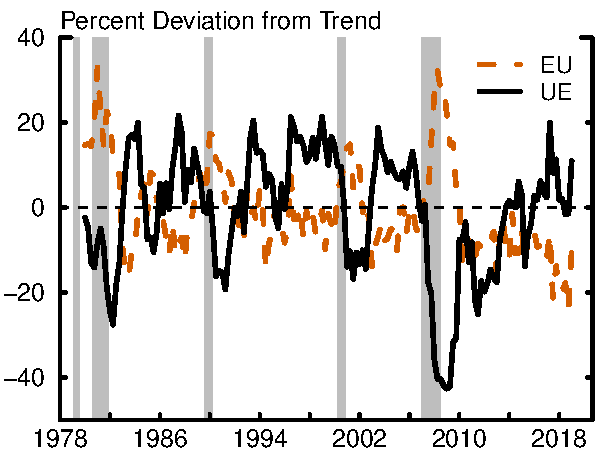
\includegraphics[scale=0.75]{flows_cyclicality_ham.pdf}
\end{subfigure}
\begin{subfigure}{.48\textwidth}
\subcaption{Gross Flows}
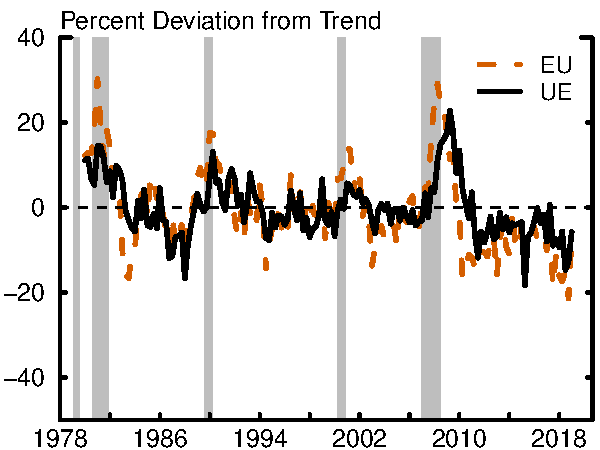
\includegraphics[scale=0.75]{grossflows_cyclicality_ham.pdf}
\end{subfigure}
\vspace{0.5cm}
\begin{adjustwidth}{0.75cm}{0.75cm}
\footnotesize Notes: Black, solid lines show $U$-to-$E$ flows. Orange, dashed lines show $E$-to-$U$ flows. Series Hamilton filtered with horizon $h$ and lag $p$ parameters set to 8 and 4 quarters, respectively. I take a quarterly average of monthly values before applying the filter. Monthly series are adjusted for seasonal variation and time aggregation bias.
\end{adjustwidth}
\end{figure}

Panel (a) shows that the $P_t(EU)$ flow probability is countercyclical while the $P_t(UE)$ flow probability is procyclical. As is well known and extensively documented in the literature, a higher fraction of employed workers lose jobs in recessions and a lower fraction of unemployed workers find jobs in recessions.

However, Panel (b) clearly indicates that both $EU_t$ and $UE_t$ gross flows are countercyclical, meaning that they rise around NBER recession dates and fall during business-cycle expansions. Therefore, the \textit{total number} of workers exiting unemployment, somewhat counterintuitively, rises in recessions. An earlier literature that examined the cyclicality of worker flows also recognized this pattern \citep{Darby:1986aa, Davis:1987aa, Blanchard:1990aa, Ritter:1993aa}. Hearkening back to the findings of this literature, Figure \ref{fig:grossflows_cyclicality} shows that the amplitude of fluctuations in $EU_t$ is greater than that of $UE_t$. Importantly, these patterns place restrictions on the macroeconomic forces that generate a rise in the unemployment rate during recessions \citep{Fujita:2011aa, Mercan:2024aa}.

\subsection{Cross-Correlations of Flow Probabilities}

I now investigate the lead-lag structure among flow probabilities and the unemployment rate. To do so, I compute cross-correlations of these variables at different horizons. In particular, I calculate the correlation coefficient between some variable $X_t$ and some other variable $Y_{t + j}$, where I allow $j$ to vary between -8 and 8 quarters and use a uniform sample size across different values of $j$. Figure \ref{fig:crosscorr_flows} contains the results of this exercise.

\begin{figure}[t!]
\centering
\caption{Cross-Correlations of Flow Probabilities and Unemployment}\label{fig:crosscorr_flows}
\begin{subfigure}{.32\textwidth}
\subcaption{$P_t(UE)$ and $P_{t + j}(EU)$}\label{fig:crosscorr_flows_a}\vspace{-0.25cm}
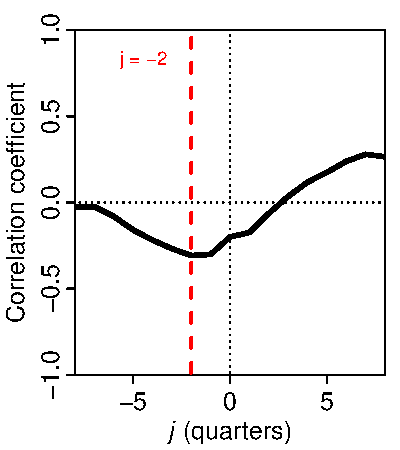
\includegraphics[scale=0.75]{flows_crosscorr_ue_eu_ham.pdf}
\end{subfigure}
\begin{subfigure}{.32\textwidth}
\subcaption{$u_t$ and $P_{t + j}(EU)$}\label{fig:crosscorr_flows_b}\vspace{-0.25cm}
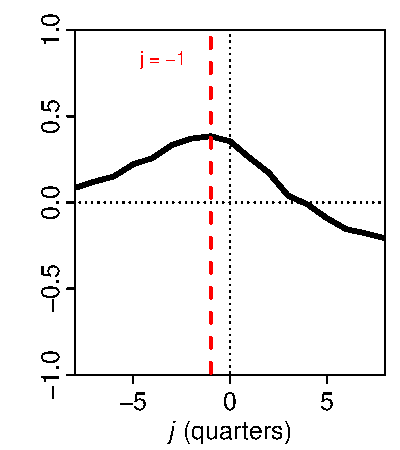
\includegraphics[scale=0.75]{flows_crosscorr_ur_eu_ham.pdf}
\end{subfigure}
\begin{subfigure}{.32\textwidth}
\subcaption{$u_t$ and $P_{t + j}(UE)$}\label{fig:crosscorr_flows_c}\vspace{-0.25cm}
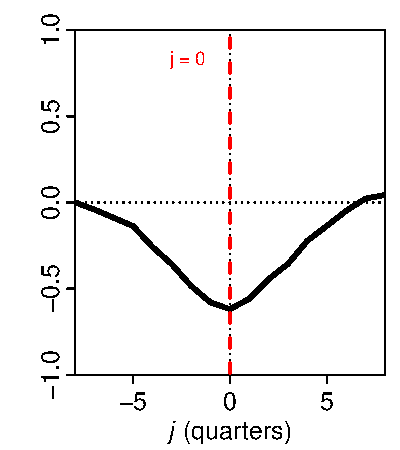
\includegraphics[scale=0.75]{flows_crosscorr_ur_ue_ham.pdf}
\end{subfigure}
\vspace{0.25cm}
\begin{adjustwidth}{0.75cm}{0.75cm}
\footnotesize Notes: Series Hamilton-filtered with horizon $h$ and lag $p$ parameters set to 8 and 4 quarters, respectively. I take a quarterly average of monthly values before applying the filter. Monthly series are adjusted for seasonal variation and time aggregation bias. Correlation coefficient is the Kendall rank correlation coefficient. Sample = 1980Q4--2017Q4.  
\end{adjustwidth}
\end{figure}

Focusing first on the left panel of Figure \ref{fig:crosscorr_flows_a}, the black, solid line shows that the unemployment-to-employment flow probability $P(UE)$ is negatively correlated with the employment-to-unemployment flow probability $P(EU)$, on average. Times when it is easier to find a job are times when a lower fraction of workers exit employment and vice versa. However, the correlation is not constant across different horizons. In particular, the red, dashed line shows that it reaches a low point at $j=-2$ quarters, indicating that $P(UE)$ is most strongly (negatively) correlated with previous values of $P(EU)$. Therefore, $P(EU)$ leads $P(UE)$ in time.

In the center panel, Figure \ref{fig:crosscorr_flows_b} shows that a similar pattern exists in the relationship between the unemployment rate ($u$) and $P(EU)$. The cross-correlation between these two variables troughs at a value of $j = -1$ quarter. Therefore, movements in the $E$-to-$U$ flow probability also lead movements in the unemployment rate. Lastly, turning to the right panel, Figure \ref{fig:crosscorr_flows_c} shows that this is not the case with the $U$-to-$E$ flow probability. Instead, the minimum correlation between $u$ and $P(UE)$ occurs at $j$ = 0. Therefore, the \textit{contemporaneous} relationship between the $U$-to-$E$ flow probability and unemployment is the strongest. Collectively, this evidence suggests that while changes in $U$-to-$E$ flows occur simultaneously with changes in the unemployment rate, changes in $E$-to-$U$ flows predate changes in the unemployment rate.

\subsection{Granger Causality in Gross Flows}

Next, I further explore the dynamic structure of worker flows by conducting a formal test of whether certain labor market flows Granger-cause others. In order to test whether some time series variable $x_t$ Granger-causes some other time series variable $y_t$, I estimate the following two equations by OLS for a given lag length $L$.\footnote{The in-sample $F$-test I implement is formalized in \cite{Hamilton:1994aa} Chapter 11.2, pages 304--305.}
\begin{align}
y_t = \ & \alpha_0 + \alpha_1 y_{t-1} + \alpha_2 y_{t-2} + \dots + \alpha_L y_{t-L} \ + \ \beta_1 x_{t-1} + \beta_2 x_{t-2} + \dots + \beta_L x_{t-L} + u_t \label{eqn:granger1} \\
y_t = \ & \gamma_0  + \gamma_1 y_{t-1} + \gamma_2 y_{t-2} + \dots + \gamma_p y_{t-L} + e_t \label{eqn:granger2}
\end{align}

\begin{table}[t!]
\centering
\caption{Does $EU_t$ Granger Cause $UE_t$?}\label{tab:granger_eu_ue}
\begin{threeparttable}\small
\begin{tabular}{c c c c c c c c c c}
\toprule
& \multicolumn{4}{c}{Raw Data} & & \multicolumn{4}{c}{Hamilton-Filtered Data} \\\cline{2-5}\cline{7-10}
& & & & & & & & &\\[-0.35cm]
& $L = 1$ & $L = 2$ & $L = 3$ & $L = 4$ & & $L = 1$ & $L = 2$ & $L = 3$ & $L = 4$\\ \hline
& & & & & & & & &\\[-0.35cm]
\input{\inputpath granger_table_eu_ue.tex}
\bottomrule
\end{tabular}
\begin{tablenotes}[para,flushleft]\footnotesize
Notes: Raw Data are quarterly averages of monthly values. Hamilton-Filtered Data are quarterly averages of monthly values, then Hamilton-filtered with quarterly parameters $h = 8$ and $p = 4$. Significance level $\alpha$ = 1\%. Sample = 1979Q4--2019Q4.
\end{tablenotes}
\end{threeparttable}
\end{table}

Then, I conduct an $F$-test of the null hypothesis $ H_0: \beta_1 = \beta_2 = \dots = \beta_L = 0 $. This tests whether the variable $x_t$ is important in predicting values of $y_t$ in a forecasting sense. If $x_t$ Granger-causes $y_t$, then information contained in $x_t$ will be useful in forecasting $y_t$ above and beyond the information contained in past values of $y_t$. To implement the test, I construct the test statistic below
$$S_1 \equiv \frac{(RSS_0 - RSS_1)/L}{RSS_1/(T-2L-1)} $$
where $RSS_1 = \sum_{t=1}^T \hat u_t^2$ is the sum of squared residuals from the regression in Equation (\ref{eqn:granger1}), $RSS_0 = \sum_{t=1}^T \hat e_t^2$ is the sum of squared residuals from the regression in Equation (\ref{eqn:granger2}), and $T$ is the number of time periods in the sample. I compare the value of the test statistic to the critical value from the $F$ distribution with parameters $L$ and $T-2L-1$.

Table \ref{tab:granger_eu_ue} displays the results of this exercise using the gross flows data, where $EU_t$ is the $x$ variable (independent variable) and $UE_t$ is the $y$ variable (dependent variable) in the unrestricted regression, Equation (\ref{eqn:granger1}). I choose a significance level of $\alpha$ = 1\% and report the test statistic, critical value, and $p$-value of the test, as well as whether the test rejects the null hypothesis. Note that under the null hypothesis, the independent variable \textit{does not} Granger-cause the dependent variable. If the test rejects the null hypothesis, then $EU_t$ is said to Granger-cause $UE_t$. I report the results of the test using several different lag lengths as well as using raw or filtered data. I also report the Bayesian information criteria (BIC) value for each lag length, which favors a value of $L=2$ in the filtered data. I find overwhelming support for the result that $EU_t$ Granger-causes $UE_t$, with $p$-values indistinguishable from 0 in most instances. 

\begin{table}[t!]
\centering
\caption{Does $UE_t$ Granger Cause $EU_t$?}\label{tab:granger_ue_eu}
\begin{threeparttable}\small
\begin{tabular}{c c c c c c c c c c}
\toprule
& \multicolumn{4}{c}{Raw Data} & & \multicolumn{4}{c}{Hamilton-Filtered Data} \\\cline{2-5}\cline{7-10}
& & & & & & & & &\\[-0.35cm]
& $L = 1$ & $L = 2$ & $L = 3$ & $L = 4$ & & $L = 1$ & $L = 2$ & $L = 3$ & $L = 4$\\ \hline
& & & & & & & & &\\[-0.35cm]
\input{\inputpath granger_table_ue_eu.tex}
\bottomrule
\end{tabular}
\begin{tablenotes}[para,flushleft]\footnotesize
Notes: Raw Data are quarterly averages of monthly values. Hamilton-Filtered Data are quarterly averages of monthly values, then Hamilton-filtered with quarterly parameters $h = 8$ and $p = 4$. Significance level $\alpha$ = 1\%. Sample = 1979Q4--2019Q4.
\end{tablenotes}
\end{threeparttable}
\end{table}

On the other hand, $UE_t$ gross flows do not appear to Granger cause $EU_t$ gross flows. Table \ref{tab:granger_ue_eu} reports the results of the test using $UE_t$ as the independent variable and $EU_t$ as the dependent variable. Across lag lengths and filtering methods considered, the null hypothesis of no Granger-causality is not rejected for the given significance level. Therefore, although the two series exhibit a very high contemporaneous correlation, a clear lead-lag structure exists between them. Namely, the number of workers exiting employment into unemployment ($EU$) Granger-causes the number of workers exiting unemployment into employment ($UE$). 

%%%%%%%%%%%%%%%%%%%%%%%%%%%%%%%%%%%%%%%%%%%%%%
% Identifying Unemployment Shocks %%%%%%%%%%%%%%%%%%%%%%%%%%%
%%%%%%%%%%%%%%%%%%%%%%%%%%%%%%%%%%%%%%%%%%%%%%
\section{Identifying Unemployment Shocks}\label{sec:empirics}

The evidence presented in Section \ref{sec:motivation} motivates a particular identification strategy of the business cycle shocks that affect unemployment. Namely, the dynamic structure of worker flows suggests that disturbances both to the unemployment rate and to unemployment outflows affect unemployment inflows only with a lag. Hence, I impose zero restrictions on the impact response of the job separation rate to disturbances in the unemployment rate and the job finding rate. I supplement these zero restrictions with additional sign restrictions and estimate shocks to labor market variables following the methodology of \cite{Arias:2018aa}. The subsections below detail the setup of the empirical model and the identification strategy.

\subsection{Model Setup}

Consider the empirical VAR model in reduced-form as follows
\begin{equation}\label{eqn:var}
y_t = b_0 + \sum_{l = 1}^L B_l y_{t-l} + \mu_t 
\end{equation}
where $y_t$ is a $(k \times 1)$ vector of endogenous variables at time $t$, $b_0$ is a $(k \times 1)$ vector of intercept terms, $B_l$ is a $(k \times k)$ matrix of coefficients for each lag length $l$, $L$ is the total number of lags in the system, and $\mu_t$ is a $(k \times 1)$ vector of reduced-form residuals at time $t$. Assume that $\mu_t \sim \mathcal{N}(0,\Sigma)$, so that the residuals are normally distributed, with mean zero and $(k \times k)$ variance-covariance matrix $\Sigma$. Moreover, assume that the vector of reduced-form residuals $\mu_t$ is related to the $(k \times 1)$ vector of structural shocks $\varepsilon_t$ in the following manner: 
\begin{equation}\label{eqn:shocks}
\mu_t = A \varepsilon_t
\end{equation}
Here, it is assumed that $\varepsilon_t \sim \mathcal{N}(0,I)$ so that the structural shocks are normally distributed, with mean zero, unit variance, and zero cross-correlation. $A$ is a $(k \times k)$ matrix referred to as the ``impact matrix'' because it captures the immediate effect that structural shocks $\varepsilon_t$ have on the endogenous variables in $y_t$.

Identifying the above system requires placing restrictions on the matrix $A$ such that the structural shocks $\varepsilon_t$ can be recovered from the reduced-form residuals $\mu_t$. Note that due to the relationship between $\varepsilon_t$ and $\mu_t$, the following holds: $\Sigma = \Var(\mu_t) = \Var(A\varepsilon_t) = A\Var(\varepsilon_t)A^\prime = A I A^\prime = AA^\prime$. Therefore, since the matrix $\Sigma$ is symmetric, it is sufficient to place $k(k-1)/2$ restrictions on the matrix $A$ in order to identify the structural shocks in Equation (\ref{eqn:shocks}). I now turn to the method I use to set these restrictions and how they relate to the motivating evidence in Section \ref{sec:motivation}.

\subsection{Identification Strategy}

I consider a four-variable system with the job separation probability $X_t$, the job finding probability $F_t$, the unemployment rate $u_t$, and average unemployment duration $d_t$, in that order. The ordering of the variables in the VAR is motivated by the evidence discussed in Section \ref{sec:motivation}. In particular, the job separation probability leads both the job finding probability and the unemployment rate. This motivates the use of zero impact restrictions on how shocks to these variables affect $X_t$.

However, since there are 4 variables in the model, the system requires additional identifying restrictions.\footnote{See the discussion in Section 2.2 of \cite{Arias:2018aa}.} I appeal to the relationship between worker flows and the distribution of unemployment duration to impose these additional restrictions. Consider a decrease in the job finding probability. All else equal, the unemployment rate will rise because of the reduced flow of workers out of the unemployment pool. Additionally, since workers face a lower probability of leaving unemployment, they remain in the unemployment pool for longer. Therefore, shocks to the job finding probability cause the unemployment rate and average unemployment duration to move in the \text{same} direction.

Consider an increase in the job separation probability. All else equal, the unemployment rate will rise because of the increased flow of workers into the unemployment pool. Additionally, since these workers have an unemployment duration of 0 by construction, the mean of the unemployment duration distribution must fall. Therefore, shocks to the job separation probability cause the unemployment rate and average unemployment duration to move in \text{opposite} directions.

For a similar reason, I also restrict the impact response of average unemployment duration to be negative following a (positive) shock to the unemployment rate. The logic of this restriction mirrors that of the response of average unemployment duration to a shock to job separation. I think of shocks to the unemployment rate holding both the job separation and job finding rates constant as capturing changes in the unemployment pool resulting from movements into and out of the labor force. Workers who join unemployment from not-in-the-labor-force ($NU$ flows) also have 0 unemployment duration by construction, leading to a fall in average unemployment duration.

\begin{table}[t!]
\centering
\caption{Identifying Restrictions}\label{tab:zero_sign_restrictions}
\begin{threeparttable}
\begin{tabular}{l c c c c}
\toprule
& Inflow & Outflow & Level & Length \\\hline
& & & & \\[-0.25cm]
Job separation probability & $+$ & $0$ & $0$ & \\
Job finding probability & & $-$ & & \\
Unemployment rate & $+$ & $+$ & $+$ & \\
Average unemployment duration & $-$ & $+$ & $-$ & $+$ \\
\bottomrule
\end{tabular}
\begin{tablenotes}[para,flushleft]\footnotesize
Notes: As suggested by \cite{Arias:2018aa}, all restrictions are imposed on impact. 
\end{tablenotes}
\end{threeparttable}
\end{table}

Table \ref{tab:zero_sign_restrictions} summarizes these restrictions. In total, I identify four shocks, which I label as shocks to the Unemployment Inflow, Unemployment Outflow, Unemployment Level, and Unemployment Length. Note that I also impose regularity conditions (along the diagonal) such that the shocks are contractionary. For instance, a shock to the unemployment outflow leads to a fall in the job finding probability.

\subsection{Estimation}

I use quarterly data on $X_t$, $F_t$, $u_t$, and $d_t$ from 1948Q1 to 2019Q4 and include 4 lags of the endogenous variables in my baseline specification.\footnote{The BIC suggests using more than 12 lags, which would increase the computational load considerably. I show in Appendix \ref{app:sec:robustness} that results are robust to using 8 lags in the system. I have also estimated the system using 1, 4, and 12 lags and found similar results.} As discussed in Section \ref{sec:data}, using the two-state model to measure the job finding and job separation probabilities allows for a larger sample, whereas worker flow series from the three-state model are only available since 1978Q1. I take quarterly averages of monthly values and filter the data using the \cite{Hamilton:2018aa} filter with the suggested quarterly parameters, $h = 8$ and $p = 4$. This ensures that the data are all expressed in the same units: percentage deviations from their respective trends.

Because my identification strategy uses a combination of zero and sign restrictions, I implement the methodology developed in \cite{Arias:2018aa} to estimate the shocks. The procedure involves drawing the reduced form coefficients $B_l$, the variance-covariance matrix of the residuals $\Sigma$, and an orthogonal rotation matrix $Q$ that maps the structural shocks into the reduced form residuals, and keeping draws of these matrices if the resulting impulse response functions satisfy the sign and zero restrictions. In particular, conditional on a draw of $(B_l,\Sigma)$, the zero restrictions impose linear restrictions on the columns of $Q$. Then, conditional on $(B_l,\Sigma,Q)$ that satisfies the zero restrictions, one checks to see if the sign restrictions are satisfied and discards the draw if they are not. I use \textit{conjugate} priors such that the prior and posterior densities come from the same family of distributions. The draws of $(B_l, \Sigma)$ are from a normal-inverse-Wishart distribution and the draws of $Q$ are from a uniform distribution, conditional on $(B_l,\Sigma)$. I implement the algorithm in Matlab using 10,000 draws.\footnote{I make use of existing Matlab codes from the Empirical Macro Toolbox \citep{Ferroni:2025aa}. See \cite{Ferroni:2025ab} for a guide to the toolbox.} 

%%%%%%%%%%%%%%%%%%%%%%%%%%%%%%%%%%%%%%%%%%%%%%
% The Effects of Unemployment Shocks %%%%%%%%%%%%%%%%%%%%%%%%%
%%%%%%%%%%%%%%%%%%%%%%%%%%%%%%%%%%%%%%%%%%%%%%
\section{The Effects of Unemployment Shocks}\label{sec:results}

I now discuss the estimated effects of the unemployment shocks on the variables in the VAR system. Then, I use local projection methods to estimate the effects of these shocks on auxiliary labor market variables. I discuss how the estimated responses of the auxiliary variables shed light on the underlying forces at work. Next, I formally decompose the variance of each variable in the system into the components accounted for by each shock. Lastly, I compute the forecast error variance decomposition (FEVD) and historical decomposition (HD) for specific recessionary episodes and discuss their implications.

\subsection{Response to Unemployment Inflow and Outflow Shocks}

\begin{figure}[t!]
\centering
\caption{Response to Unemployment Inflow Shock}\label{fig:ir_eu}
\begin{subfigure}{.47\textwidth}
\centering
\subcaption{Job Separation Probability}\vspace{-0.1cm}

\includegraphics[scale=0.675]{zerosign/zerosign_ir_v1_e1.pdf}
\end{subfigure}
\vspace{0.35cm}
\begin{subfigure}{.47\textwidth}
\centering
\subcaption{Job Finding Probability}\vspace{-0.1cm}

\includegraphics[scale=0.675]{zerosign/zerosign_ir_v2_e1.pdf}
\end{subfigure}
\vspace{0.35cm}
\begin{subfigure}{.47\textwidth}
\centering
\subcaption{Unemployment Rate}\vspace{-0.1cm}

\includegraphics[scale=0.675]{zerosign/zerosign_ir_v3_e1.pdf}
\end{subfigure}
\begin{subfigure}{.47\textwidth}
\centering
\subcaption{Average Unemployment Duration}\vspace{-0.1cm}

\includegraphics[scale=0.675]{zerosign/zerosign_ir_v4_e1.pdf}
\end{subfigure}
\begin{adjustwidth}{0.5cm}{0.5cm}
\footnotesize Notes: Response to a one standard deviation (contractionary) structural shock. Units are percentage deviations from trend. Black, solid lines display the median response. Dark gray bands represent the 68\% credible set. Light gray bands represent the 90\% credible set.
\end{adjustwidth}
\end{figure}

Figure \ref{fig:ir_eu} contains the estimated impulse response functions to a shock to the first variable in the VAR system. I label this shock an ``unemployment inflow'' shock, as it is associated with the job separation probability. The job separation probability rises by about 5\% on impact and then remains elevated relative to trend for almost two years. The job finding probability falls slightly on impact, troughs at about -2\% after 2--3 quarters, and then slowly returns to trend. The unemployment rate displays a hump-shaped pattern in that it initially rises, peaks about 4 quarters after the shock, and then subsequently returns to trend. Note that the response of the unemployment rate is driven by the joint dynamics of the job separation and job finding probabilities. An initial spike in job separations causes the unemployment rate to increase on impact; it then rises further because of the decrease in the job finding probability. Average unemployment duration initially falls because of a spike in unemployment inflows, but subsequently rises as workers accumulate in the unemployment pool and the job finding probability falls.

\begin{figure}[t!]
\centering
\caption{Response to Unemployment Outflow Shock}\label{fig:ir_ue}
\begin{subfigure}{.47\textwidth}
\centering
\subcaption{Job Separation Probability}\vspace{-0.1cm}

\includegraphics[scale=0.675]{zerosign/zerosign_ir_v1_e2.pdf}
\end{subfigure}
\vspace{0.35cm}
\begin{subfigure}{.47\textwidth}
\centering
\subcaption{Job Finding Probability}\vspace{-0.1cm}

\includegraphics[scale=0.675]{zerosign/zerosign_ir_v2_e2.pdf}
\end{subfigure}
\vspace{0.35cm}
\begin{subfigure}{.47\textwidth}
\centering
\subcaption{Unemployment Rate}\vspace{-0.1cm}

\includegraphics[scale=0.675]{zerosign/zerosign_ir_v3_e2.pdf}
\end{subfigure}
\begin{subfigure}{.47\textwidth}
\centering
\subcaption{Average Unemployment Duration}\vspace{-0.1cm}

\includegraphics[scale=0.675]{zerosign/zerosign_ir_v4_e2.pdf}
\end{subfigure}
\begin{adjustwidth}{0.5cm}{0.5cm}
\footnotesize Notes: Response to a one standard deviation (contractionary) structural shock. Units are percentage deviations from trend. Black, solid lines display the median response. Dark gray bands represent the 68\% credible set. Light gray bands represent the 90\% credible set.
\end{adjustwidth}
\end{figure}

Figure \ref{fig:ir_ue} shows the response of the variables in the system to a (contractionary) shock to the second variable in the system, the job finding probability, which I label a ``unemployment outflow'' shock. Recall that under my identification assumptions, an unemployment outflow shock may not affect the job separation probability on impact. In response to this shock, there is not a significant reaction of the job separation probability at any horizon, though separations do rise slightly in the first 1--4 quarters under the median impulse response function. The job finding probability falls on impact and slowly returns to trend, meaning that an initial fall in unemployment outflows has a persistent effect on the rate at which workers find jobs out of unemployment. Both the unemployment rate and the average unemployment duration rise significantly on impact and remain elevated for several quarters relative to trend.

\subsection{Response to Unemployment Level and Length Shocks}

\begin{figure}[t!]
\centering
\caption{Response to Unemployment Level Shock}\label{fig:ir_ur}
\begin{subfigure}{.47\textwidth}
\centering
\subcaption{Job Separation Probability}\vspace{-0.1cm}

\includegraphics[scale=0.675]{zerosign/zerosign_ir_v1_e3.pdf}
\end{subfigure}
\vspace{0.35cm}
\begin{subfigure}{.47\textwidth}
\centering
\subcaption{Job Finding Probability}\vspace{-0.1cm}

\includegraphics[scale=0.675]{zerosign/zerosign_ir_v2_e3.pdf}
\end{subfigure}
\vspace{0.35cm}
\begin{subfigure}{.47\textwidth}
\centering
\subcaption{Unemployment Rate}\vspace{-0.1cm}

\includegraphics[scale=0.675]{zerosign/zerosign_ir_v3_e3.pdf}
\end{subfigure}
\begin{subfigure}{.47\textwidth}
\centering
\subcaption{Average Unemployment Duration}\vspace{-0.1cm}

\includegraphics[scale=0.675]{zerosign/zerosign_ir_v4_e3.pdf}
\end{subfigure}
\begin{adjustwidth}{0.5cm}{0.5cm}
\footnotesize Notes: Response to a one standard deviation (contractionary) structural shock. Units are percentage deviations from trend. Black, solid lines display the median response. Dark gray bands represent the 68\% credible set. Light gray bands represent the 90\% credible set.
\end{adjustwidth}
\end{figure}

Figure \ref{fig:ir_ur} shows the response of the variables in the system to a contractionary shock to the third variable in the system, the unemployment rate, which I label a ``unemployment level'' shock. This shock captures movements in the unemployment rate that occur despite fixed job separation and job finding probabilities. Therefore, I argue that this shock reflects movements into and out of the labor force that affect the size of the unemployment pool, but initially leave inflow and outflow rates unchanged. For instance, this shock would capture cyclical changes in labor supply incentives \citep{Graves:2024aa}.

From the figure, we can see that unemployment level shocks are not associated with large, significant changes in the job separation or job finding probability. If anything, the median impulse response shows that the job finding probability falls modestly (by about 1\%) following a positive unemployment length shock. Consistent with the interpretation that this shock represents an increase in the size of the unemployment pool all else equal, this finding points to the presence of congestion externalities that are a hallmark of search and matching models. 

\begin{figure}[t!]
\centering
\caption{Response to Unemployment Length Shock}\label{fig:ir_ud}
\begin{subfigure}{.47\textwidth}
\centering
\subcaption{Job Separation Probability}\vspace{-0.1cm}

\includegraphics[scale=0.675]{zerosign/zerosign_ir_v1_e4.pdf}
\end{subfigure}
\vspace{0.35cm}
\begin{subfigure}{.47\textwidth}
\centering
\subcaption{Job Finding Probability}\vspace{-0.1cm}

\includegraphics[scale=0.675]{zerosign/zerosign_ir_v2_e4.pdf}
\end{subfigure}
\vspace{0.35cm}
\begin{subfigure}{.47\textwidth}
\centering
\subcaption{Unemployment Rate}\vspace{-0.1cm}

\includegraphics[scale=0.675]{zerosign/zerosign_ir_v3_e4.pdf}
\end{subfigure}
\begin{subfigure}{.47\textwidth}
\centering
\subcaption{Average Unemployment Duration}\vspace{-0.1cm}

\includegraphics[scale=0.675]{zerosign/zerosign_ir_v4_e4.pdf}
\end{subfigure}
\begin{adjustwidth}{0.5cm}{0.5cm}
\footnotesize Notes: Response to a one standard deviation (contractionary) structural shock. Units are percentage deviations from trend. Black, solid lines display the median response. Dark gray bands represent the 68\% credible set. Light gray bands represent the 90\% credible set.
\end{adjustwidth}
\end{figure}

Lastly, Figure \ref{fig:ir_ud} shows the responses to a positive shock to the final variable in the system, average unemployment duration, which I label a ``unemployment length'' shock. Again, the interpretation of this shock warrants additional discussion. I think of unemployment length shocks as capturing \textit{compositional} changes in the pool of unemployed workers that shift the average of the distribution of unemployment duration, but that initially leave unemployment inflows, outflows, and levels unchanged. This could reflect time-varying selection, on either observed or unobserved characteristics, in the types of workers that comprise the pool of unemployment that affects the average propensity for workers to eventually \textit{leave} unemployment \citep{Ahn:2022aa, Gregory:2025aa}. In other words, unemployment length shocks capture changes in the average of the unemployment duration distribution holding total unemployment fixed. 

The figure shows that I do not find large, significant responses of the other variables in the system to unemployment length shocks, on average. However, as discussed below, this does not preclude them from being important in driving unemployment dynamics during specific recessionary episodes.

\subsection{Responses of Other Labor Market Variables}

Exploring the effects of the identified unemployment shocks on additional variables helps to unpack the underlying structural forces these shocks capture. I therefore use local projection methods \citep{Jorda:2005aa} to estimate the impact of unemployment inflow and outflow shocks on auxiliary labor market variables. Let $\hat \varepsilon^i_t$ represent an identified shock to variable $i$ at time $t$. To recover the time series of $\hat \varepsilon^i_t$'s, I invert the impact matrix for each draw of a rotation matrix that satisfies my identification strategy and back out the structural shocks according to Equation \ref{eqn:shocks}. Then, I estimate the equation
\begin{equation}\label{eqn:lp}
x_{t+h} = \alpha_h + \beta_h \hat \varepsilon^i_t + e_{t+h}
\end{equation}
for different horizons $h$ and for different outcome variables $x_{t+h}$. The coefficients $\beta_h$ capture the response of the outcome variable to the shock at horizon $h$, providing an estimate of the impulse response function \citep{Plagborg:2021aa}. I then plot the median responses and associated confidence intervals in the figures below.

I examine the responses of $U$-to-$E$ gross flows, $E$-to-$U$ gross flows, and vacancies to unemployment inflow and outflow shocks. As shown in Figure \ref{fig:grossflows_cyclicality}, both gross flow series are countercyclical, so shocks that are associated with large recessionary increases in unemployment should also lead to increases in gross worker flows. The response of job openings is informative about the degree to which my estimated shocks generate Beveridge Curve dynamics, which has been a central focus of the search-and-matching literature. Collectively, examining these auxiliary impulse responses also serves as a check on the validity of the identification approach. 

\begin{figure}[t!]
\centering
\caption{Response to Unemployment Inflow Shock}\label{fig:lp_eu}
\begin{subfigure}{.32\textwidth}
\subcaption{$E$-to-$U$ Gross Flow}\vspace{-0.1cm}
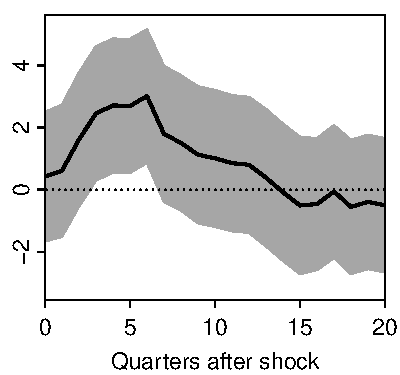
\includegraphics[scale=0.75]{zerosign/zerosign_lp_x1_e1.pdf}
\end{subfigure}
\begin{subfigure}{.32\textwidth}
\subcaption{$U$-to-$E$ Gross Flow}\vspace{-0.1cm}
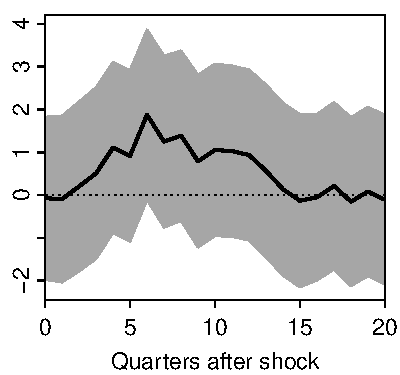
\includegraphics[scale=0.75]{zerosign/zerosign_lp_x2_e1.pdf}
\end{subfigure}
\begin{subfigure}{.32\textwidth}
\subcaption{Vacancies}\vspace{-0.1cm}
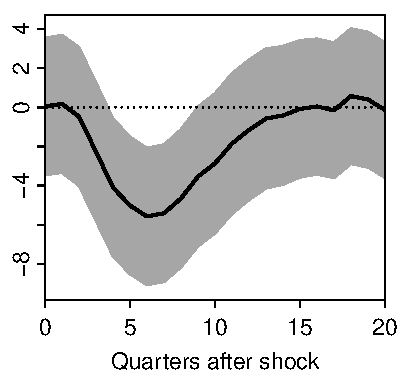
\includegraphics[scale=0.75]{zerosign/zerosign_lp_x3_e1.pdf}
\end{subfigure}
\vspace{0.5cm}
\begin{adjustwidth}{0.5cm}{0.5cm}
\footnotesize Notes: Gross flow series constructed as described in Section \ref{sec:data}. Vacancy series is the help-wanted index from \cite{Barnichon:2010aa}. Black, solid lines show the median response and gray bands show the median 95\% confidence interval. Dependent variables are in log-levels, so units are percent changes.
\end{adjustwidth}
\end{figure}

Figure \ref{fig:lp_eu} plots the response of gross flows and vacancies to a contractionary unemployment inflow shock. After an increase in unemployment inflows, the total number of workers moving from employment to unemployment (left panel) initially rises. It then increases to a peak change of almost 3\% around 6 quarters before returning to its initial level. The gross flow of workers between unemployment and employment (center panel) does not change on impact, but eventually rises by just under 2\%, also peaking around 6 quarters after the shock. Note that these patterns are consistent with the evidence presented in Figure \ref{fig:grossflows_cyclicality}; both $EU$ and $UE$ gross flows rise in contractionary periods. Lastly, vacancies decline considerably in response to a contractionary unemployment inflow shock, falling by almost over 6\% a year after the shock. This pattern is consistent with not only a decline in labor market tightness during a recession (as the unemployment rate also rises), but also the decrease in the job finding probability in response to an inflow shock shown in Figure \ref{fig:ir_eu}. In sum, unemployment inflow shocks are associated with the observed behavior of labor market variables during a recession.

\begin{figure}[t!]
\centering
\caption{Response to Unemployment Outflow Shock}\label{fig:lp_ue}
\begin{subfigure}{.32\textwidth}
\subcaption{$E$-to-$U$ Gross Flow}\vspace{-0.1cm}
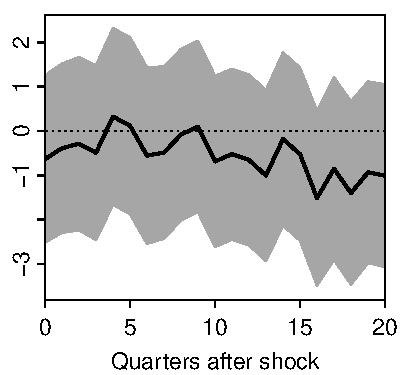
\includegraphics[scale=0.75]{zerosign/zerosign_lp_x1_e2.pdf}
\end{subfigure}
\begin{subfigure}{.32\textwidth}
\subcaption{$U$-to-$E$ Gross Flow}\vspace{-0.1cm}
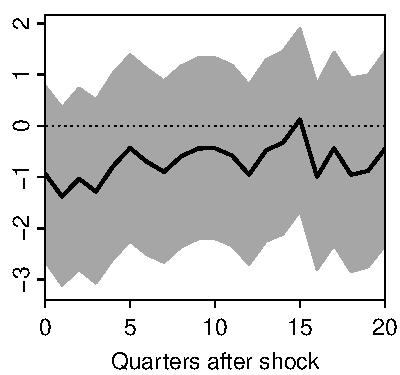
\includegraphics[scale=0.75]{zerosign/zerosign_lp_x2_e2.pdf}
\end{subfigure}
\begin{subfigure}{.32\textwidth}
\subcaption{Vacancies}\vspace{-0.1cm}
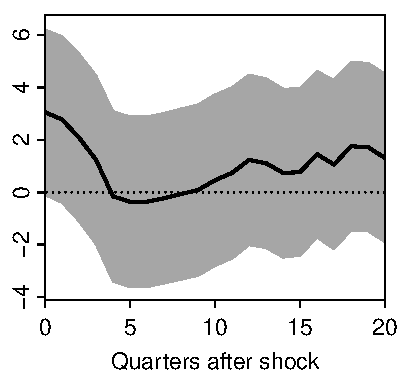
\includegraphics[scale=0.75]{zerosign/zerosign_lp_x3_e2.pdf}
\end{subfigure}
\vspace{0.5cm}
\begin{adjustwidth}{0.5cm}{0.5cm}
\footnotesize Notes: Gross flow series constructed as described in Section \ref{sec:data}. Vacancy series is the help-wanted index from \cite{Barnichon:2010aa}. Black, solid lines show the median response and gray bands show the median 95\% confidence interval. Dependent variables are in log-levels, so units are percent changes.
\end{adjustwidth}
\end{figure}

Figure \ref{fig:lp_ue} plots the responses of the same three variables to an unemployment outflow shock. In contrast, unemployment outflow shocks do not seem to replicate the empirical patterns referenced above. Neither response is meaningfully large at the given level of statistical significance. The same is true of the response of vacancies, as the estimated impulse response function is not significant for any horizon. Therefore, unemployment inflow shocks are more promising candidates for generating realistic unemployment dynamics, as they are consistent with both the cyclical behavior of gross worker flows and Beveridge Curve dynamics.\footnote{Appendix \ref{app:sec:figures} shows that both $EU$ and $UE$ gross flows increase somewhat in response to unemployment level shocks, but not to length shocks. Vacancies do not react significantly to either unemployment level or unemployment length shocks.}

\subsection{Contribution to Unemployment Volatility}

I now assess the contribution of each structural shock to the volatility of unemployment. To do so, I compute the variance of each of the endogenous variables under specific shock combinations. I derive a closed-form expression for the variance of the variables in a $VAR(p)$ model as a function of the VAR coefficients and structural shocks in Appendix \ref{app:sec:proofs} and utilize the formulas for the results in this section.

Let $\Var(y_t | \varepsilon^i_t)$ denote the variance of the variables in the vector $y_t$ under a particular structural shock $\varepsilon^i_t$. The total variance of $y_t$ is equal to the sum across $i$ of $\Var(y_t | \varepsilon^i_t)$ because the structural shocks are independent. Therefore, we can decompose the variance of each endogenous variable into the components accounted for by each structural shock. This procedure is similar in spirit to the forecast error variance decomposition (FEVD), which I discuss below, but it does not fix a particular horizon.

\begin{table}[t!]
\centering
\caption{Shock Contribution to Endogenous Variable Variance}\label{tab:shock_contribution}
\begin{threeparttable}\small
\begin{tabular}{l | c c c c | c}
\toprule
& Inflow & Outflow & Level & Length & Total \\\hline
& & & & & \\[-0.25cm]
\input{\inputpath zerosign_var_decomp.tex}
\bottomrule
\end{tabular}
\begin{tablenotes}[para,flushleft]\footnotesize
Notes: Each element of the table contains the percentage of the overall variance of a given variable explained by a particular shock under the median of the estimated coefficients. Total column shows the sum across the Inflow, Outflow, Level, and Length columns.
\end{tablenotes}
\end{threeparttable}
\end{table}

Table \ref{tab:shock_contribution} shows the results of this decomposition for each variable in my baseline specification. As noted above, summing across the structural shocks returns the overall variance of the endogenous variables, so the columns sum to 100\% by construction. Focusing first on the the unemployment inflow shock, we can see that it explains a large fraction of each of the variables in the system. It naturally explains a large portion of the variance of the job separation probability, but also plays a large role in the variance of the job finding probability and average unemployment duration. This is because, as discussed above, job finding falls and average unemployment duration eventually rises substantially in response to an increase in unemployment inflows (Figure \ref{fig:ir_eu}). Unemployment outflow shocks also play a considerable role in changes in the job finding probability and average unemployment duration.

Next, the row corresponding to the unemployment rate shows that the unemployment inflow shock primarily explains the variance of the unemployment rate. In particular, unemployment inflow shocks account for about 45\% of unemployment rate fluctuations, while unemployment outflow shocks account for only about 15\%, closer to the contributions of the other two shocks. It would therefore be tempting to conclude from this decomposition alone that job separation (the ``ins'' of unemployment) plays a larger role in unemployment fluctuations than job finding (the ``outs'' of unemployment). However, this decomposition also relies on the \textit{endogenous} responses of the variables in the VAR system, which confound the roles played individually by the job finding and job separation probabilities. I therefore derive an additional decomposition to separate their contributions.

\paragraph{Shutting Down Interaction} Table \ref{tab:shock_contribution_noint} shows the results from the same decomposition, shutting down interaction effects between the job finding and job separation probabilities. In particular, I set the VAR coefficients on lags of $F_t$ in the $X_t$ equation and on lags of $X_t$ in the $F_t$ equation to 0.\footnote{Note that I do not set the own-lags in the VAR system to 0, so past lags of the job separation rate may still affect the current job separation rate. Figure \ref{fig:ir_eu} shows that the response of the separation rate to its own shock is highly persistent, largely explaining why the inflow shock still plays an out-sized role in this decomposition.} If part of the large role of unemployment inflow shocks in the variance of the unemployment rate is due to the endogenous, negative response of the job finding probability, we should see a smaller role for these shocks in unemployment fluctuations. The third row of the table shows that this is indeed the case, where the contribution of unemployment inflow (outflow) shocks decreases (increases) from 45\% (15\%) to 35\% (18\%). Note that in percentage terms, both of these changes are similar in magnitude, about 20\% in either case. Clearly, the interaction between job finding and job separation affects any conclusions drawn about the contribution of both margins to unemployment rate movements.

\begin{table}[t!]
\centering
\caption{Shock Contribution to Endogenous Variable Variance, No Interaction}\label{tab:shock_contribution_noint}
\begin{threeparttable}\small
\begin{tabular}{l | c c c c | c}
\toprule
& Inflow & Outflow & Level & Length & Total \\\hline
& & & & & \\[-0.25cm]
\input{\inputpath zerosign_var_decomp_noint.tex}
\bottomrule
\end{tabular}
\begin{tablenotes}[para,flushleft]\footnotesize
Notes: Each element of the table contains the percentage of the overall variance of a given variable explained by a particular shock under the median of the estimated coefficients, with the interaction between job finding and job separation turned off. Total column shows the sum across the Inflow, Outflow, Level, and Length columns.
\end{tablenotes}
\end{threeparttable}
\end{table}

The results of these decompositions caution against the interpretation that changes in the job finding probability are solely or primarily responsible for fluctuations in the unemployment rate. Whereas \cite{Shimer:2012aa} finds that the contribution of job finding is 2-3 times larger than the contribution of job separation to unemployment volatility, my results are more in line with those of \cite{Fujita:2009aa}, who find that job separations explain between 40 and 50\% of fluctuations in unemployment. I find that while the job separation probability has a quantitatively larger contribution, both margins play a substantial role in driving unemployment dynamics. Moreover, allowing for job separations to dynamically affect job finding changes the conclusions regarding the contribution of each margin to overall unemployment volatility. 

\subsection{Forecast Error Variance Decomposition}

I also compute the forecast error variance decomposition (FEVD) to further explore the role of the shocks at different horizons. Figure \ref{fig:fevd} plots this decomposition for the main variables of interest: the job separation probability, the job finding probability, and the unemployment rate. As is also apparent from Table \ref{tab:shock_contribution}, unemployment inflow shocks play a large role in driving unemployment dynamics. The left panel shows that they contribute to over 90\% of fluctuations in the job separation probability in a 5-year window. The remaining 10\% are attributed to unemployment length shocks, which are associated with innovations to average unemployment duration. This result likely stems from the inverse relationship between job separations and the unemployment duration distribution. Times when workers are flowing into unemployment are times when average unemployment duration is falling and vice versa.

\begin{figure}[t!]
\centering
\caption{Forecast Error Variance Decomposition}\label{fig:fevd}
\begin{subfigure}{.47\textwidth}
\centering
\subcaption{Job Separation Probability}\vspace{-0.1cm}
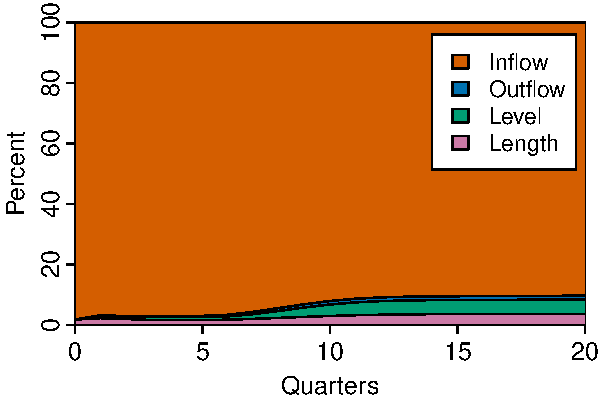
\includegraphics[scale=0.675]{zerosign/zerosign_fevd_v1.pdf}
\end{subfigure}
\vspace{0.35cm}
\begin{subfigure}{.47\textwidth}
\centering
\subcaption{Job Finding Probability}\vspace{-0.1cm}
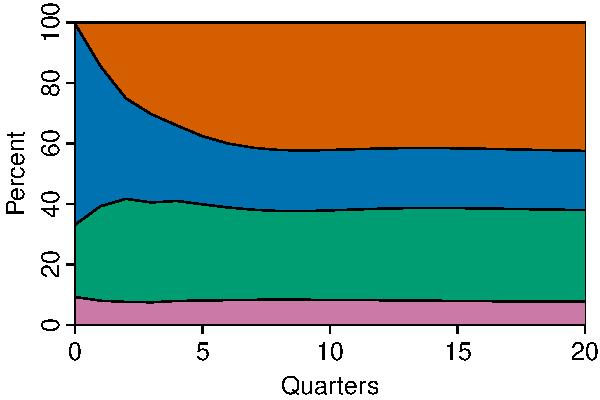
\includegraphics[scale=0.675]{zerosign/zerosign_fevd_v2.pdf}
\end{subfigure}
\vspace{0.35cm}
\begin{subfigure}{.47\textwidth}
\centering
\subcaption{Unemployment Rate}\vspace{-0.1cm}
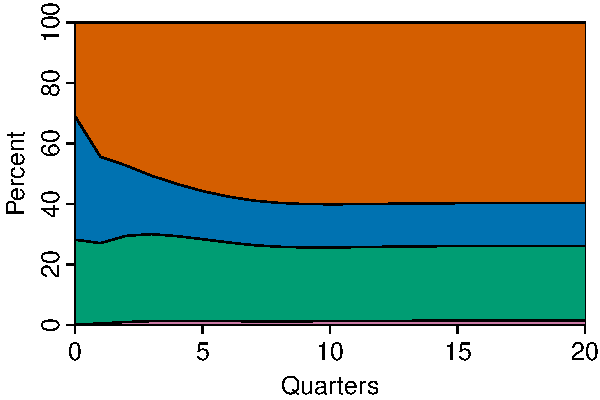
\includegraphics[scale=0.675]{zerosign/zerosign_fevd_v3.pdf}
\end{subfigure}
\begin{subfigure}{.47\textwidth}
\centering
\subcaption{Average Unemployment Duration}\vspace{-0.1cm}
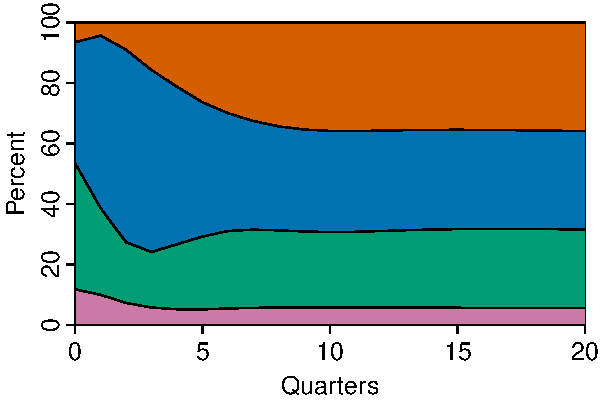
\includegraphics[scale=0.675]{zerosign/zerosign_fevd_v4.pdf}
\end{subfigure}
\begin{adjustwidth}{0.5cm}{0.5cm}
\footnotesize Notes: Figure shows the percentage of the unpredictable component of each variable accounted for by different shocks across horizons, calculated using pointwise median impulse response functions.
\end{adjustwidth}
\end{figure}

The other panels of Figure \ref{fig:fevd} show that unemployment inflow shocks also drive the bulk of both job finding and unemployment fluctuations, but their contribution changes significantly across horizons. Indeed, unemployment \textit{outflow} shocks play a significant role in both job finding and unemployment changes at shorter horizons. They comprise the majority share of job finding probability fluctuations at shorter horizons (1-4 quarters), a pattern masked by the results presented in Table \ref{tab:shock_contribution}. At longer horizons, however, unemployment inflow shocks dominate. The large contribution of these shocks at longer horizons results from the endogenous response of the job finding probability to an unemployment inflow shock (Figure \ref{fig:ir_eu}), whereby the job finding probability falls for several quarters following a spike in $E$-to-$U$ flows. The FEVD also makes clear that while both job finding and job separation play an important role in unemployment fluctuations in an \textit{accounting} sense, it is \textit{shocks} to unemployment inflows that are quantitatively more relevant. Identifying innovations in worker flows therefore serves to distinguish the two margins, providing a more complete picture of the forces responsible for driving the business-cycle dynamics of unemployment.

Lastly, note that unemployment level shocks are important in explaining movements in the job finding probability, unemployment rate, and average unemployment duration across all horizons. This indicates that movements into and out of the labor force are also a quantitatively relevant feature of cyclical labor market dynamics \citep{Elsby:2015aa}.

\subsection{Historical Decomposition}

Lastly, I assess the contribution of unemployment shocks to labor market dynamics during different historical episodes. While the variance decomposition and forecast error variance decomposition show that unemployment inflow shocks play a larger role than unemployment outflow shocks on average, their contributions may not be constant across recessions. Each U.S. recession has been driven by a different combination of macroeconomic disturbances. Because my identified unemployment shocks likely capture a confluence of underlying structural forces, they should also display different roles in different economic downturns. I therefore compute the historical decomposition (HD) and compare the role of unemployment inflow and outflow shocks in the 2001 and 2008 recessions.

Figure \ref{fig:hd_2001} plots the HD for the 2001 recession. From the top-left panel, we can see that unemployment inflow shocks primarily drove changes in the job separation probability, consistent with the results above. However, the top-right panel reveals that both unemployment inflow and unemployment outflow shocks played a large role in driving job finding dynamics in this recession. Early in the recession, unemployment outflow shocks accounted for the majority share of the sharp drop in the job finding probability. After the end of the recession according to the NBER recession dates (shown in dark, gray bars in the figure), both unemployment inflow and outflow shocks accounted for a depressed job finding probability into the early stages of recovery. As the job finding probability recovered after 2002, the role of unemployment inflow shocks diminished, disappearing almost completely by the end of 2003. 

\begin{figure}[t!]
\centering
\caption{Historical Decomposition, 2001 Recession}\label{fig:hd_2001}
\begin{subfigure}{.47\textwidth}
\centering
\subcaption{Job Separation Probability}\vspace{-0.1cm}
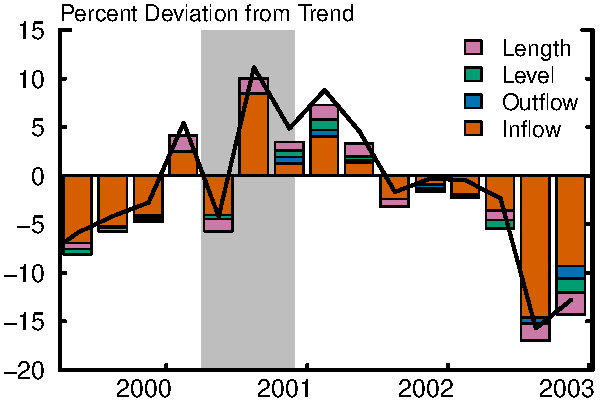
\includegraphics[scale=0.675]{zerosign/zerosign_hd_v1_2001.pdf}
\end{subfigure}
\vspace{0.35cm}
\begin{subfigure}{.47\textwidth}
\centering
\subcaption{Job Finding Probability}\vspace{-0.1cm}\label{fig:hd_2001_ue}
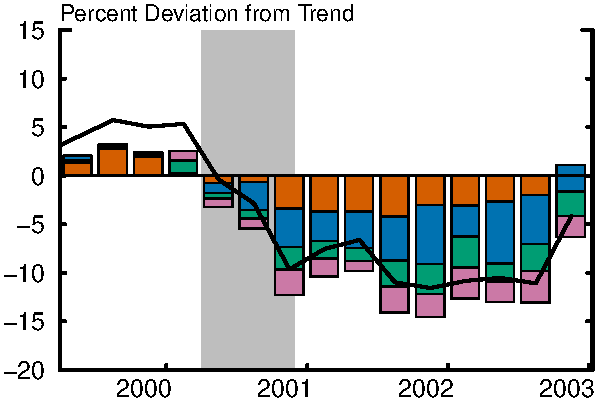
\includegraphics[scale=0.675]{zerosign/zerosign_hd_v2_2001.pdf}
\end{subfigure}
\vspace{0.35cm}
\begin{subfigure}{0.47\textwidth}
\centering
\subcaption{Unemployment Rate}\vspace{-0.1cm}
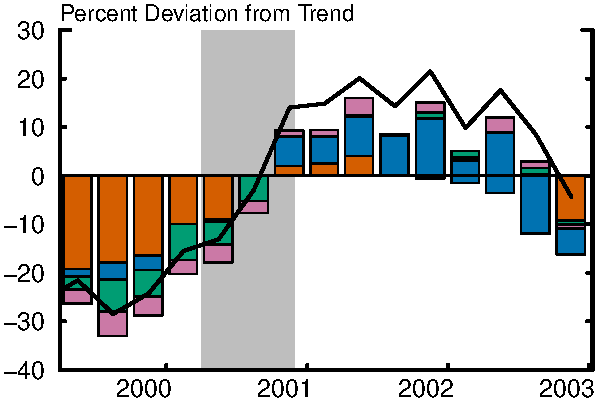
\includegraphics[scale=0.675]{zerosign/zerosign_hd_v3_2001.pdf}
\end{subfigure}
\begin{subfigure}{0.47\textwidth}
\centering
\subcaption{Average Unemployment Duration}\vspace{-0.1cm}
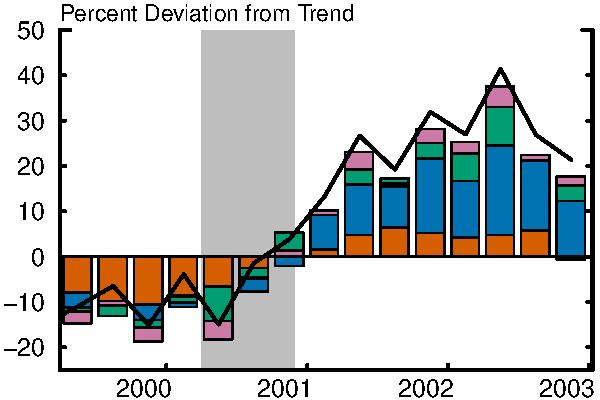
\includegraphics[scale=0.675]{zerosign/zerosign_hd_v4_2001.pdf}
\end{subfigure}
\begin{adjustwidth}{0.5cm}{0.5cm}
\footnotesize Notes: Figure shows shock contribution to the evolution of each variable, calculated by taking the median HD across draws. Black, solid line shows the actual level of the given variable, which may not line up exactly due to the contribution of the initial condition.
\end{adjustwidth}
\end{figure}

Turning to the bottom-left panel, we can see that unemployment outflow shocks accounted for the largest portion of the increase in the unemployment rate during this period. While unemployment inflow shocks also played a role, their contribution becomes negligible by the end of 2002. Lastly, the bottom-right panel shows that unemployment outflow shocks also explain the bulk of changes in average unemployment duration during this time horizon. Moreover, unemployment length shocks played a relatively small role. Collectively, this indicates that the decrease in the job finding probability (and corresponding increase in average unemployment duration) reflects the diminished re-employment prospects for workers \textit{across} the unemployment distribution rather than large compositional changes in the unemployment pool. Overall, the results of this exercise show that the 2001 recession was characterized more so by a depressed job finding rate (for all types of workers) than by an increased separation rate. The same may not apply to \textit{all} recessions, however.

\begin{figure}[t!]
\centering
\caption{Historical Decomposition, 2008 Recession}\label{fig:hd_2008}
\begin{subfigure}{.47\textwidth}
\centering
\subcaption{Job Separation Probability}\vspace{-0.1cm}
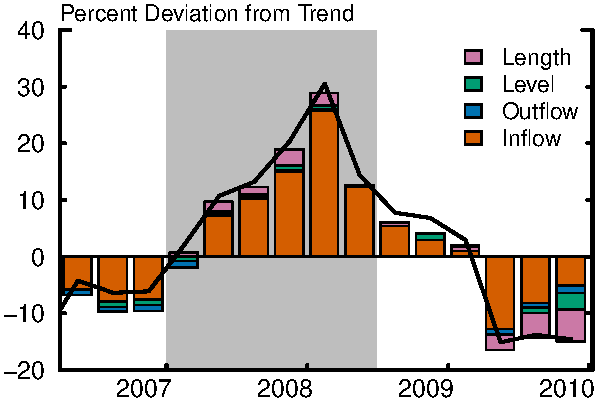
\includegraphics[scale=0.675]{zerosign/zerosign_hd_v1_2008.pdf}
\end{subfigure}
\vspace{0.35cm}
\begin{subfigure}{.47\textwidth}
\centering
\subcaption{Job Finding Probability}\vspace{-0.1cm}\label{fig:hd_2008_ue}
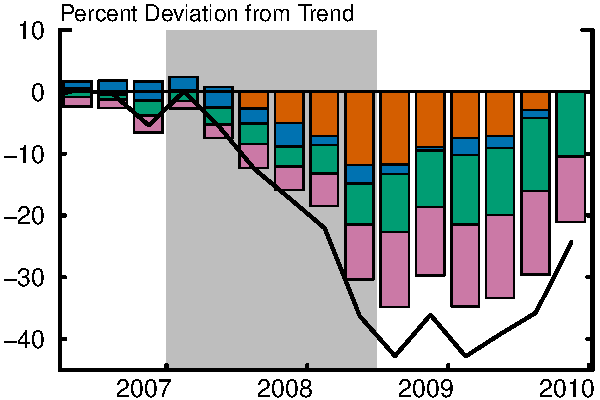
\includegraphics[scale=0.675]{zerosign/zerosign_hd_v2_2008.pdf}
\end{subfigure}
\vspace{0.35cm}
\begin{subfigure}{0.47\textwidth}
\centering
\subcaption{Unemployment Rate}\vspace{-0.1cm}
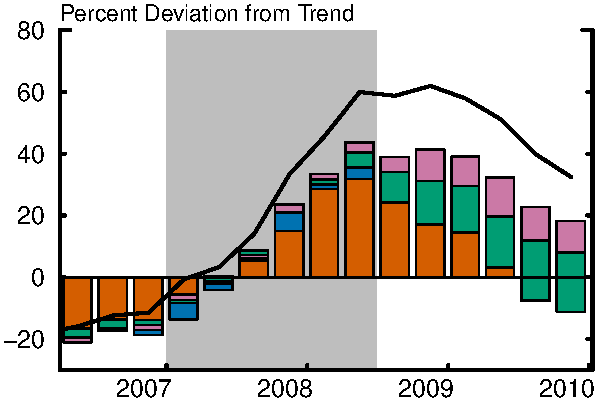
\includegraphics[scale=0.675]{zerosign/zerosign_hd_v3_2008.pdf}
\end{subfigure}
\begin{subfigure}{0.47\textwidth}
\centering
\subcaption{Average Unemployment Duration}\vspace{-0.1cm}
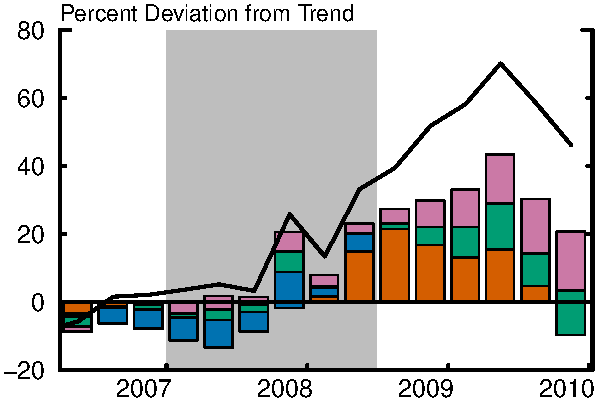
\includegraphics[scale=0.675]{zerosign/zerosign_hd_v4_2008.pdf}
\end{subfigure}
\begin{adjustwidth}{0.5cm}{0.5cm}
\footnotesize Notes: Figure shows shock contribution to the evolution of each variable, calculated by taking the median HD across draws. Black, solid line shows the actual level of the given variable, which may not line up exactly due to the contribution of the initial condition.
\end{adjustwidth}
\end{figure}

For instance, Figure \ref{fig:hd_2008} shows that the opposite conclusion holds for the 2008 recession. Unemployment inflow shocks accounted for a large share of fluctuations in the job separation probability, job finding probability, and unemployment rate during this period. As discussed, this is because they endogenously lead to drops in the job finding probability, putting further upward pressure on the unemployment rate. This recession was characterized by a large and persistent increase in the unemployment rate and a slow recovery. The historical decomposition of this period reveals that this was due to elevated unemployment inflows and the associated decline in the speed with which unemployed workers found new jobs. 

Next, we can also see that unemployment length shocks were an important driver of labor market dynamics during the 2008 recession, particularly for the job finding probability. This result indicates that compositional changes in the pool of unemployed workers put downward pressure on the \textit{average} job finding propensity, either directly or by reducing job creation incentives for firms.\footnote{For instance, if firms have a difficult time screening out bad matches during a recession \citep{Engbom:2021aa}.}

Interestingly, unemployment level shocks also played a large role in unemployment dynamics during this period. I interpret these shocks as capturing any forces that result in changes in the unemployment rate holding both $E$-to-$U$ flows and $U$-to-$E$ flows constant. For instance, they may capture movements into and out of the labor force. Their large role in unemployment fluctuations during the 2008 recession and subsequent recovery makes sense in the context of the large decline in labor force participation during this period. Indeed, the right panel shows that they had become the dominant force in driving the unemployment rate by the end of 2010.

Collectively, this analysis reveals that studying the role of unemployment inflows and unemployment outflows in conjunction paints a more accurate picture of labor market dynamics. Though the variance decomposition exercises above revealed that unemployment inflow shocks are the quantitatively dominant force on average, they played drastically different roles in different recessions. Moreover, assessing the endogenous response of labor market variables to unemployment shocks is crucial for understanding their effects. Therefore, focusing only on a particular margin of worker flows may lead to misleading conclusions about unemployment fluctuations.

%%%%%%%%%%%%%%%%%%%%%%%%%%%%%%%%%%%%%%%%%%%%%%
% Implications for Models of the Labor Market %%%%%%%%%%%%%%%%%%%%%%
%%%%%%%%%%%%%%%%%%%%%%%%%%%%%%%%%%%%%%%%%%%%%%
\section{Implications for Models of the Labor Market}\label{sec:implications}

I now discuss the implications of my empirical results for theoretical models of search and unemployment in labor markets. First, I briefly discuss the various underlying forces that my crude structural shock estimates likely capture. 

\subsection{Discussion of Structural Shocks}

Though I refer to the recovered unemployment inflow, outflow, level, and length shocks as ``structural shocks,'' I do not think of them as fundamental, underlying macroeconomic disturbances. Rather, they are attempts to isolate changes in labor market variables that are plausibly exogenous to prevailing economic conditions. They encompass the responses of worker flows and unemployment to deeper changes in the aggregate economy, but in this sense, studying the response of labor market variables to these shocks is informative about what underlying structural forces are at play. 

For instance, a job separation (unemployment inflow) shock likely captures classic structural shocks such as productivity, monetary policy, or credit supply shocks that result in sudden changes in employment exits without an \textit{immediate} effect on job finding because of frictions in the hiring process. At the microeconomic level, contractionary shocks of this variety lead to sharp contractions in firms' desired employment levels. Because firms face adjustment costs on the hiring margin, they typically adjust to changes in desired employment levels through the separation margin.\footnote{For this reason, \cite{Haltiwanger:2018ab} argue that the \textit{change} in the unemployment rate is a more reliable indicator of the state of the business cycle, as it better aligns with NBER recession dates as well as credit crunches. Changes in the unemployment rate during the initial phases of a recession are more likely to be driven by changes in the separation margin, consistent with the results in this paper and others.}

Similarly, since unemployment outflow shocks only affect job separations with a lag, they likely capture changes in worker search incentives (search effort) that do not have an immediate effect on overall labor demand. Indeed, I do not find that they produce significant movements in the job separation rate at any horizon (Figure \ref{fig:ir_ue}). However, they do contribute significantly to unemployment volatility over the business cycle, in line with studies that argue that countercyclical worker search effort plays an important role in shaping unemployment fluctuations \citep{Mukoyama:2018aa, Graves:2024aa}.

Next, I think of unemployment level shocks as capturing forces that affect the unemployment rate, holding both inflow and outflow rates fixed. For instance, my preferred interpretation is that unemployment level shocks primarily capture changes in the participation margin, which also plays a crucial role in unemployment fluctuations \citep{Elsby:2015aa}. Indeed, I find in my decomposition exercises that these shocks account for about a quarter of all unemployment fluctuations, on average, and were particularly important during the Great Recession, which saw a large and persistent drop in labor force participation.

Lastly, unemployment length shocks are those that capture changes in the distribution of unemployment duration, holding inflows, outflows, and the unemployment rate constant.\footnote{Note that total unemployment can increase but the unemployment rate remain unchanged if the denominator in the unemployment rate -- the total labor force -- also increases by a proportional amount. Therefore, the incidence of an unemployment length shock does not preclude the size of the unemployed pool becoming larger, if for instance, individuals join unemployment from outside of the labor force.} Therefore, they represent compositional shifts in the different ``types'' of workers that make up the pool of unemployment over the business cycle \citep{Ahn:2023aa, Gregory:2025aa}. More generally, I think of unemployment length shocks as capturing forces that drive a wedge between the average job finding probability and average unemployment duration. In the canonical search-and-matching framework, one is the inverse of the other. However, it is well known that the job finding rate displays \textit{duration dependence} such that workers with shorter unemployment durations are more likely to exit unemployment than those at longer durations \citep{Kroft:2013aa, Ahn:2020aa, Ahn:2022aa}. My results show that these shocks were important in explaining unemployment dynamics during the recovery from the Great Recession, a period characterized by both a depressed job finding rate and elevated level of long-term unemployment.

\subsection{Theories of Unemployment}

The evidence I present in this paper shows that changes in the inflow to unemployment should not be ignored in analyzing the cyclical behavior of the labor market. The strong pattern of Granger causality that I establish in Section \ref{sec:motivation} suggests that countercyclical $E$-to-$U$ flows help give rise to unemployment fluctuations. My empirical methodology formalizes the role of job separations in driving unemployment, and I find that job separation shocks have a large and significant contribution to unemployment volatility. Therefore, treating job separations as exogenous and acyclical in models of the labor market misses one of the key factors responsible for increased unemployment in recessions.

In terms of economic modeling, my paper suggests a return to the considerations that motivated the original \cite{Mortensen:1994aa} study. These authors included an endogenous separation margin in their model exactly to explain the rise in unemployment inflows at the beginning of an economic downturn. However, in subsequent analyses, the endogenous separation margin largely dropped out of this class of models and focus turned instead to explaining what factors determine fluctuations in the job finding rate.\footnote{For example, \cite{Gavazza:2018aa} motivate their study on labor market matching efficiency by stating ``Swings in the job-finding rate account for the bulk of unemployment fluctuations (Shimer 2012)''.} For instance, the model used in \cite{Shimer:2005aa}, which famously concluded that productivity shocks in the canonical search-and-matching framework cannot quantitatively generate fluctuations in labor market tightness in line with those in the data, notably does not feature endogenous separations. 

Studies that reintroduce a role for endogenous job separation find that the picture is more complicated \citep{denHann:2000aa, Fujita:2012aa}. These papers show that by making small modifications to the DMP framework, the model can capture labor market fluctuations both qualitatively and quantitatively. A recent study by \cite{Hall:2022aa} draws attention to a persistently elevated separation rate as a potential feedback mechanism to explain why unemployment falls slowly after a recession. My results support the notion that the job separation margin should be modeled explicitly in theories of unemployment.

Moreover, allowing for a dynamic interaction between job separation and job finding affects the degree to which changes in either margin contribute to the overall variance of unemployment. In my main empirical exercise, I estimate that the job finding rate does not react significantly to a unemployment inflow shock on impact and then declines persistently for several quarters, leading to a hump-shaped increase in the unemployment rate. Hence, my findings point to the presence of mechanisms that propagate an initial impulse in job separation to future movements in both job separation and job finding. Several recent papers posit channels that are consistent with this pattern, and I view my results as providing direct empirical support for the theoretical predictions in these studies \citep{Coles:2018aa,Ahn:2020aa,Engbom:2021aa,Gregory:2025aa,Mercan:2024aa}. This result in particular underscores the importance of considering mechanisms beyond endogenous separations alone. 

Ultimately, my results are in line with the conclusions of other studies that economists should jointly consider unemployment inflows and outflows. For instance, \cite{Elsby:2009aa} declare that ``everyone's a winner'' and reject attempts to analyze the two margins separately. The evidence from my study reinforces the need for macroeconomic models to explicitly incorporate the dynamic interplay between job loss and job finding in order to accurately capture the business-cycle dynamics of unemployment.

%%%%%%%%%%%%%%%%%%%%%%%%%%%%%%%%%%%%%%%%%%%%%%
%% Conclusion %%%%%%%%%%%%%%%%%%%%%%%%%%%%%%%%%%%%%
%%%%%%%%%%%%%%%%%%%%%%%%%%%%%%%%%%%%%%%%%%%%%%
\section{Conclusion}\label{sec:conclusion}

In this paper, I develop a methodology to assess how inflows to versus outflows from the pool of unemployed workers drive the dynamics of the unemployment rate. In a recession, unemployment may rise if it is harder for workers to find jobs or if more workers lose jobs. This question has been widely studied by macro and labor economists, but to my knowledge, no general consensus exists regarding which channel is more important.

My analysis uses two different types of worker flows series that measure how often workers move between employment and unemployment. While gross flows measure the total number of workers who transition between labor market states, flow probabilities measure the likelihood these transitions occur. I show that regardless of the series used, job separation precedes job finding in time. Importantly, however, the probability a worker transitions from unemployment to employment is procyclical while the gross flow of workers from unemployment to employment is countercyclical.

I estimate a VAR model under an identification strategy motivated by this evidence and use my estimates to decompose changes in the unemployment rate into the contributions of unemployment inflows and outflows. I find that while the unemployment inflow margin dominates, both margins account for a significant fraction of unemployment volatility. Unlike models of the labor market that abstract from endogenous movements in job separation, my results suggest that economists should endeavor to understand the reasons why more workers lose jobs during recessions in conjunction with the reasons why jobs become harder to find. 

%%%%%%%%%%%%%%%%%%%%%%%%%%%%%%%%%%%%%%%%%%%%%%
% AI Tools %%%%%%%%%%%%%%%%%%%%%%%%%%%%%%%%%%%%%%%%
%%%%%%%%%%%%%%%%%%%%%%%%%%%%%%%%%%%%%%%%%%%%%%
\newpage
\subsection*{Declaration of AI-assisted technologies in manuscript preparation}

During the preparation of this work, the author used ChatGPT, developed by OpenAI and accessed via a web interface (Free Tier), to assist in the following minor tasks:
\begin{itemize}
\item Checking spelling and grammar
\item Checking sentence structure and flow
\item Refactoring code (e.g. writing functions) to improve replication package structure
\end{itemize}

\noindent After using this tool/service, the author reviewed and edited the content as needed and takes full responsibility for the content of the published article.

%%%%%%%%%%%%%%%%%%%%%%%%%%%%%%%%%%%%%%%%%%%%%%
% References %%%%%%%%%%%%%%%%%%%%%%%%%%%%%%%%%%%%%%
%%%%%%%%%%%%%%%%%%%%%%%%%%%%%%%%%%%%%%%%%%%%%%
\newpage
\bibliography{unemployment-literature}

%%%%%%%%%%%%%%%%%%%%%%%%%%%%%%%%%%%%%%%%%%%%%%
% Appendix %%%%%%%%%%%%%%%%%%%%%%%%%%%%%%%%%%%%%%%
%%%%%%%%%%%%%%%%%%%%%%%%%%%%%%%%%%%%%%%%%%%%%%
\newpage
\appendix

% Restart numbering
\renewcommand\thefigure{\thesection.\arabic{figure}}    
\renewcommand\thetable{\thesection.\arabic{table}}
\renewcommand\theequation{\thesection.\arabic{equation}}
\setcounter{figure}{0}
\setcounter{table}{0}
\setcounter{equation}{0}

\section{Details on Measurement}\label{app:sec:measurement}

\subsection{IPUMS CPS Microdata}

I link survey respondents across consecutive months using the variable \texttt{CPSIDV}. This variable is constructed by IPUMS as a unique person-level identifier and includes linking criteria that ensures individuals match on age, sex, and race characteristics.\footnote{See \url{https://cps.ipums.org/cps/cps_linking_documentation.shtml} for more information on linking individuals in the IPUMS CPS data} I choose 1978 as the start of the sample because the years 1976 and 1977 contain several unlinkable months, leading to breaks in the series. After linking individuals, I use the variable \texttt{EMPSTAT} to determine whether a given individual was employed ($E$), unemployed ($U$), or not-in-the-labor-force ($N$) in a particular month. I then compute weighted counts of the number of individuals who transition across labor market states using weights (\texttt{LNKFW1MWT}) provided by IPUMS specifically designed for month-to-month linkages. 

\subsection{Time Aggregation Bias}

Let $P_t$ denote the monthly, discrete time Markov transition matrix between labor market states. In my application, this is a 3$\times$3 matrix with non-negative entries and columns that sum to 1.\footnote{Note that this is because I exclude persons with missing labor force status is either month $t$ or month $t+1$.} The continuous time counterpart to $P_t$, which I denote $\Lambda_t$, can be recovered from the formula below.
\begin{equation}
\Lambda_t = O_t N_t O_t^{-1}
\end{equation}
In this formula, $O_t$ is the matrix of eigenvectors of $P_t$ and $N_t$ is a diagonal matrix containing the \textit{natural logarithm} of the corresponding eigenvalues. Such a decomposition is possible as long as $P_t$ has distinct, real, and positive eigenvalues, which is the case in my sample and also holds in the \cite{Shimer:2012aa} data. Lastly, I construct the time aggregation adjusted, monthly, discrete time Markov transition matrix by converting the continuous time transition rates back to transition probabilities.  Let $\pi_t^{AB}$ denote an element in $\Pi_t$ and let $\lambda_t^{AB}$ denote an element in $\Lambda_t$ for two different labor market states $A$ and $B$. Then, 
\begin{equation}
\pi_t^{AB} = 1 - \exp(-\lambda_t^{AB})
\end{equation}

\subsection{Short-Term Unemployment}

The 1994 CPS redesign introduced a discontinuity in the short-term unemployment rate series $U^s_t$. Beginning in 1994, the CPS introduced dependent interviewing techniques such that only individuals in rotation groups 1 and 5, the ``incoming rotation groups,'' are asked explicitly about their unemployment duration, while unemployment duration for workers in other rotation groups is imputed. The discontinuity produces a structural break in both the job finding probability $F_t$ and the job separation probability $X_t$ in 1994 that is visible in the level of each series. Following \cite{Shimer:2012aa}, I use CPS microdata to correct for this discontinuity.\footnote{See \cite{Shimer:2012aa} Appendix A for additional detail on how to implement the correction.} I download data on unemployment duration from IPUMS CPS and keep only individuals in the incoming rotation groups. I then compute the total number of workers with unemployment duration less than 5 weeks using the appropriate sample weights. Therefore, my short-term unemployment series $U_t^s$ contains the published short-term unemployment series from the BLS before 1994, and the estimated series using CPS microdata after 1994. Appendix Figure \ref{app:fig:shimer_replication} shows both the uncorrected and corrected flow probabilities, which match those used in \cite{Shimer:2012aa}.

\subsection{Adjustment Steps}

As described in Section \ref{sec:data}, I adjust the grossflows series from the three-state model for various biases recognized by the literature. The specific sequence of steps is below.
\begin{enumerate}
\item Begin with the full 3-by-3 matrix of grossflows between labor market states: Employment ($E$), Unemployment ($U$), and Not-in-the-Labor Force ($N$). Let $N_{i,j}$ represent an element of this matrix.
\item Convert grossflows to proportions by dividing by the total population. In other words, compute: $\pi_{i,j} \equiv N_{i,j} / P$, where $P \equiv \sum_i \sum_j N_{i,j}$.
\item Interpolate any missing observations introduced by unlinkable months using the last observation carried forward (LOCF) method.
\item Seasonally adjust the resulting (non-missing) proportions using the Census Bureau's X-13ARIMA-SEATS Seasonal Adjustment Program. I use the R implementation of this program found in the \texttt{seasonal} package.
\item Compute flow probabilities $p_{i,j}$. Let $\hat \pi_{i,j}$ denote seasonally adjusted flow proportions. Then $p_{i,j} \equiv \hat\pi_{i,j} / \sum_i{\hat\pi_{i,j}}$.
\item Adjust $p_{i,j}$ for time aggregation bias as described above.
\item To recover grossflow proportions that are adjusted for time aggregation bias, I use the perpetual inventory method. I initialize the (relative) stock of workers in each state to the value published by the BLS in January 1978. I then roll forward the proportions using the probabilities calculated in step 6. 
\end{enumerate}

\subsection{Replication and Extension of Shimer (2012)}\label{app:sec:shimer_replication}

\begin{figure}[H]
\centering
\caption{Transition Probabilities in the 2-State Model}\label{app:fig:shimer_replication}
\begin{subfigure}{.45\textwidth} % Panel (a)
\subcaption{Job Finding}
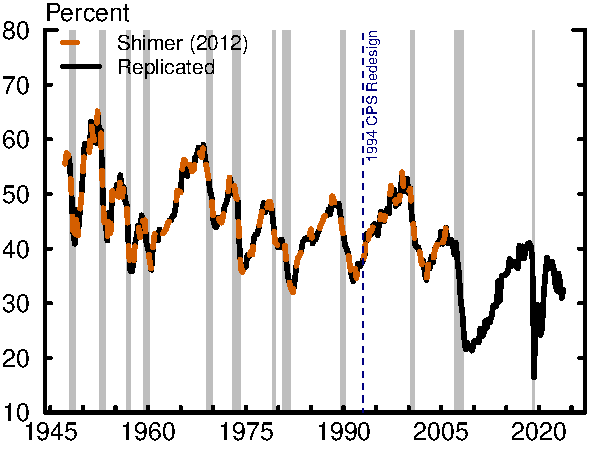
\includegraphics[scale=0.7]{shimer_2state_job_find_adj.pdf} \vspace{0.5cm}
\end{subfigure}
\begin{subfigure}{.45\textwidth} % Panel (b)
\subcaption{Employment Exit}
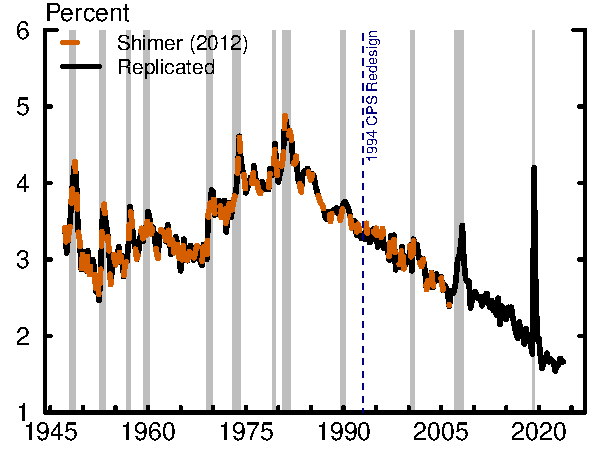
\includegraphics[scale=0.7]{shimer_2state_emp_exit_adj.pdf} \vspace{0.5cm}
\end{subfigure}
\begin{subfigure}{.45\textwidth} % Panel (c)
\subcaption{Job Finding (Uncorrected)}
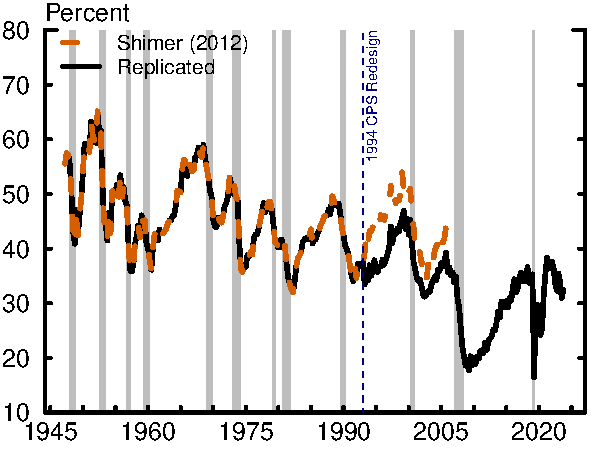
\includegraphics[scale=0.7]{shimer_2state_job_find.pdf}
\end{subfigure}
\begin{subfigure}{.45\textwidth} % Panel (d)
\subcaption{Employment Exit (Uncorrected)}
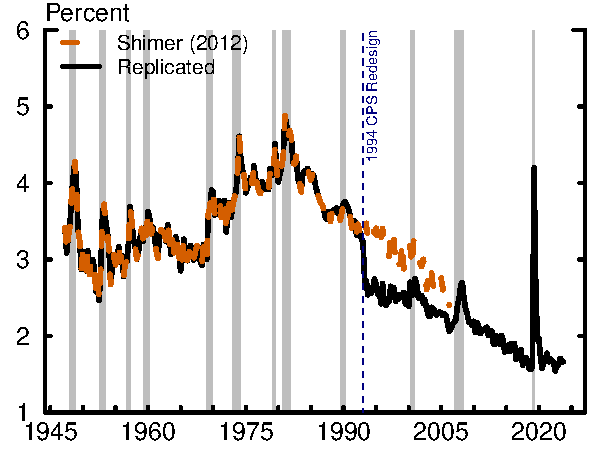
\includegraphics[scale=0.7]{shimer_2state_emp_exit.pdf}
\end{subfigure}
\vspace{0.5cm}
\begin{adjustwidth}{1cm}{1cm}
\footnotesize Notes: Black, solid lines show author's calculations based on the methodology described in Section \ref{sec:data}. Orange, dashed lines show data downloaded from Robert Shimer's website (\url{https://sites.google.com/site/robertshimer/research/flows}).
\end{adjustwidth}
\end{figure}

\begin{figure}[H]
\centering
\caption{Transition Probabilities in the 3-State Model}\label{app:fig:flows_measures}
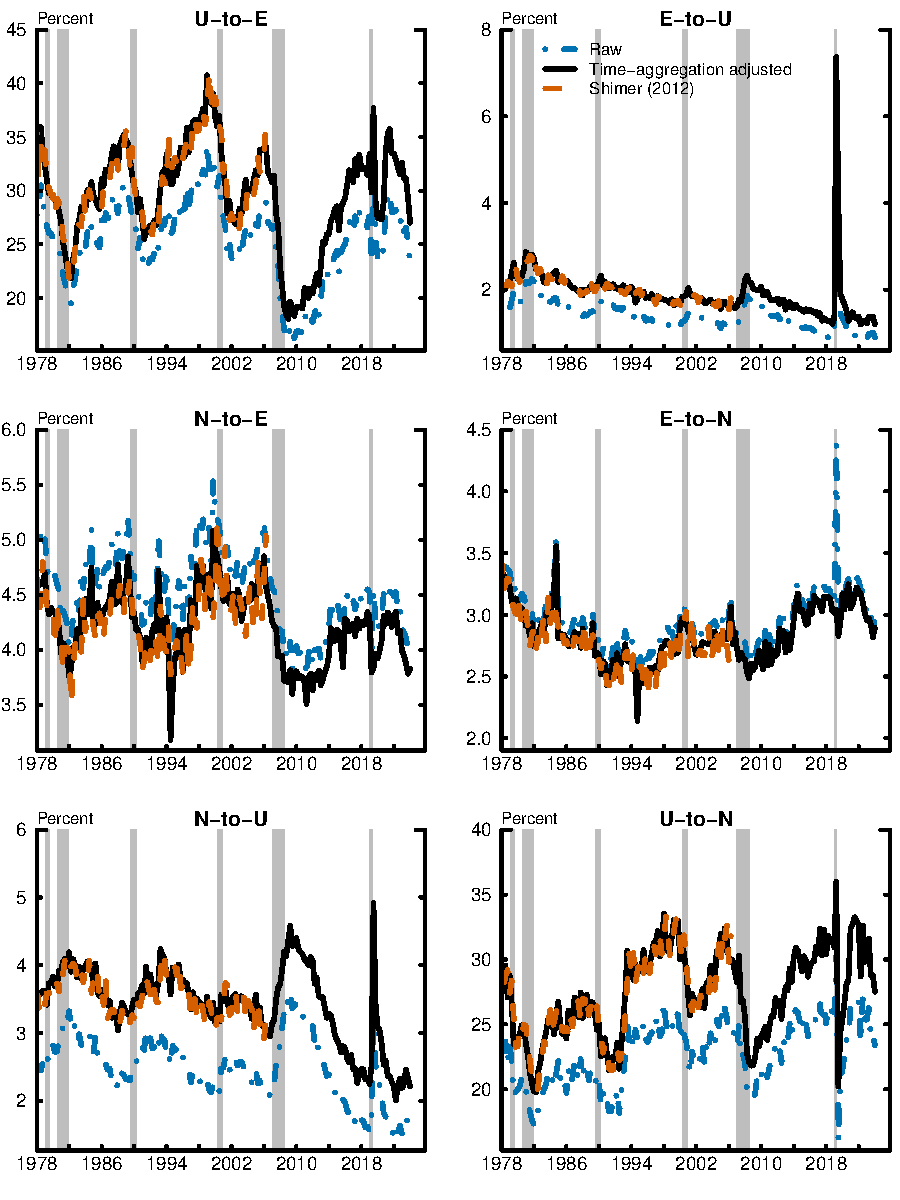
\includegraphics[scale=0.94]{shimer_3state.pdf}
\vspace{0.05cm}
\begin{adjustwidth}{1cm}{1cm}
\footnotesize Notes: Black, solid lines show author's calculations based on the methodology described in Section \ref{sec:data}. Orange, dashed lines show data downloaded from Robert Shimer's website (\url{https://sites.google.com/site/robertshimer/research/flows}). Blue, dash-dot lines show author's calculations, unadjusted for time aggregation bias.
\end{adjustwidth}
\end{figure}

\subsection{Cyclical Properties of Flows Probabilities, Different Samples}

\begin{figure}[H]
\centering
\caption{Detrended Flow Probabilities}\label{app:fig:2state_vs_3state}
\begin{subfigure}{.45\textwidth} % Panel (a)
\subcaption{$U$-to-$E$, Hamilton-Filtered}
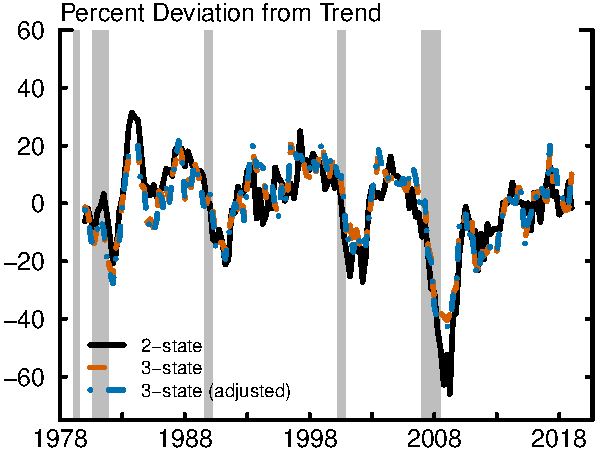
\includegraphics[scale=0.7]{2state_vs_3state_ham_ue.pdf} \vspace{0.5cm}
\end{subfigure}
\begin{subfigure}{.45\textwidth} % Panel (b)
\subcaption{$E$-to-$U$, Hamilton-Filtered}
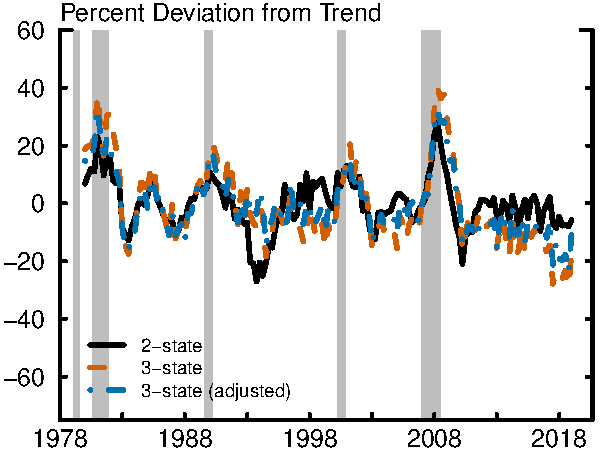
\includegraphics[scale=0.7]{2state_vs_3state_ham_eu.pdf} \vspace{0.5cm}
\end{subfigure}
\begin{subfigure}{.45\textwidth} % Panel (c)
\subcaption{$U$-to-$E$, HP-Filtered}
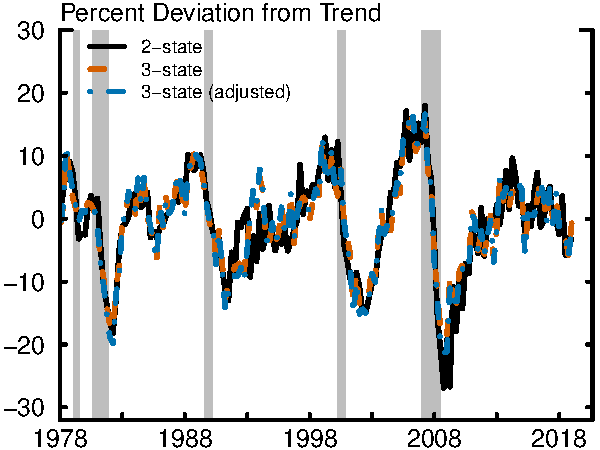
\includegraphics[scale=0.7]{2state_vs_3state_hpf_ue.pdf} \vspace{0.5cm}
\end{subfigure}
\begin{subfigure}{.45\textwidth} % Panel (d)
\subcaption{$E$-to-$U$, HP-Filtered}
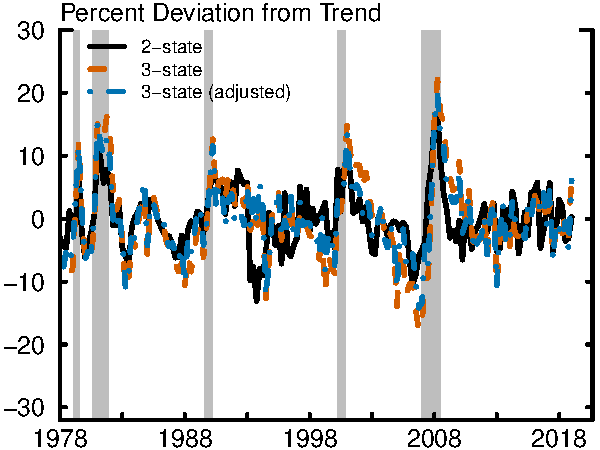
\includegraphics[scale=0.7]{2state_vs_3state_hpf_eu.pdf} \vspace{0.5cm}
\end{subfigure}
\vspace{0.05cm}
\begin{adjustwidth}{1cm}{1cm}
\footnotesize Notes: Author's calculations based on the methodology described in Section \ref{sec:data}. Black, solid lines show flow probabilities for the two-state model. Orange, dashed lines show flow probabilities for the three-state model, unadjusted for time aggregation bias. Blue, dash-dot lines show flow probabilities for the three-state model, adjusted for time aggregation bias. I take a quarterly average of monthly values before applying the respective filter. I set the horizon $h$ and lag $p$ parameters of the Hamilton filter to 8 and 4 quarters, respectively. I set the smoothing parameter of the HP filter to 1,600.
\end{adjustwidth}
\end{figure}

\newpage
\section{Additional Figures and Tables}\label{app:sec:figures}

\subsection{Local Projections}

\begin{figure}[H]
\centering
\caption{Response to Unemployment Level Shock}\label{app:fig:lp_e3}
\begin{subfigure}{.32\textwidth}
\subcaption{$E$-to-$U$ Gross Flow}\vspace{-0.1cm}
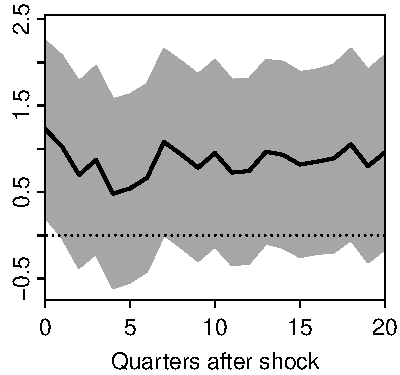
\includegraphics[scale=0.75]{zerosign/zerosign_lp_x1_e3.pdf}
\end{subfigure}
\begin{subfigure}{.32\textwidth}
\subcaption{$U$-to-$E$ Gross Flow}\vspace{-0.1cm}
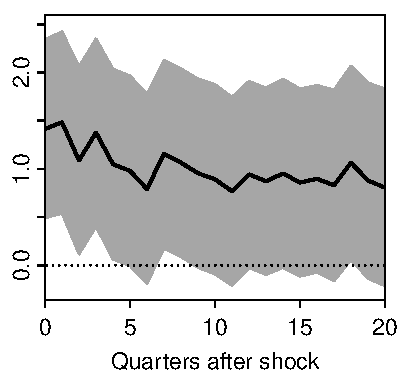
\includegraphics[scale=0.75]{zerosign/zerosign_lp_x2_e3.pdf}
\end{subfigure}
\begin{subfigure}{.32\textwidth}
\subcaption{Vacancies}\vspace{-0.1cm}
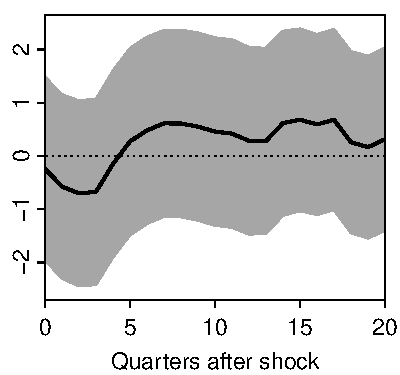
\includegraphics[scale=0.75]{zerosign/zerosign_lp_x3_e3.pdf}
\end{subfigure}
\vspace{0.5cm}
\begin{adjustwidth}{0.5cm}{0.5cm}
\footnotesize Notes: Gross flow series constructed as described in Section \ref{sec:data}. Vacancy series is the help-wanted index from \cite{Barnichon:2010aa}. Black solid lines show estimated $\beta_h$ coefficients. Gray bands show 95\% confidence intervals. Dependent variables are in log-levels so that units are percent changes.
\end{adjustwidth}
\end{figure}

\begin{figure}[H]
\centering
\caption{Response to Unemployment Length Shock}\label{app:fig:lp_e4}
\begin{subfigure}{.32\textwidth}
\subcaption{$E$-to-$U$ Gross Flow}\vspace{-0.1cm}
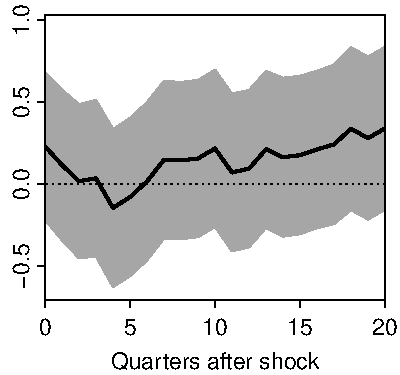
\includegraphics[scale=0.75]{zerosign/zerosign_lp_x1_e4.pdf}
\end{subfigure}
\begin{subfigure}{.32\textwidth}
\subcaption{$U$-to-$E$ Gross Flow}\vspace{-0.1cm}
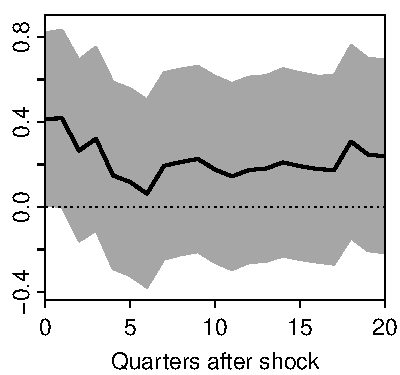
\includegraphics[scale=0.75]{zerosign/zerosign_lp_x2_e4.pdf}
\end{subfigure}
\begin{subfigure}{.32\textwidth}
\subcaption{Vacancies}\vspace{-0.1cm}
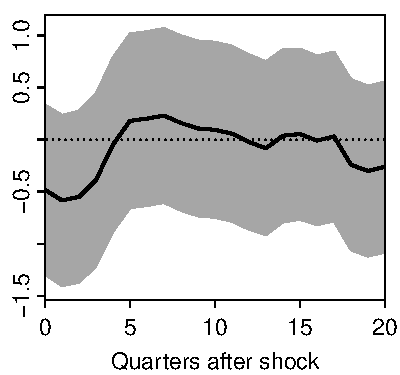
\includegraphics[scale=0.75]{zerosign/zerosign_lp_x3_e4.pdf}
\end{subfigure}
\vspace{0.5cm}
\begin{adjustwidth}{0.5cm}{0.5cm}
\footnotesize Notes: Gross flow series constructed as described in Section \ref{sec:data}. Vacancy series is the help-wanted index from \cite{Barnichon:2010aa}. Black solid lines show estimated $\beta_h$ coefficients. Gray bands show 95\% confidence intervals. Dependent variables are in log-levels so that units are percent changes.
\end{adjustwidth}
\end{figure}

\newpage
\section{Robustness}\label{app:sec:robustness}

\subsection{Motivating Evidence}

\begin{figure}[H]
\centering
\caption{Cyclical Properties of Worker Flows (HP-Filtered)}\label{app:fig:grossflows_cyclicality_hpf}
\begin{subfigure}{.48\textwidth}
\subcaption{Flow Probabilities}
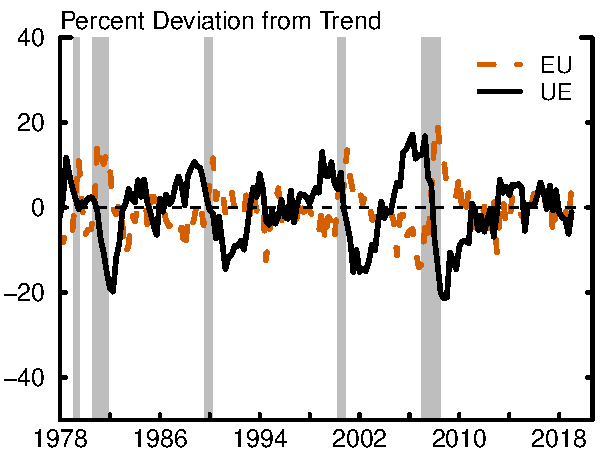
\includegraphics[scale=0.75]{flows_cyclicality_hpf.pdf}
\end{subfigure}
\begin{subfigure}{.48\textwidth}
\subcaption{Gross Flows}
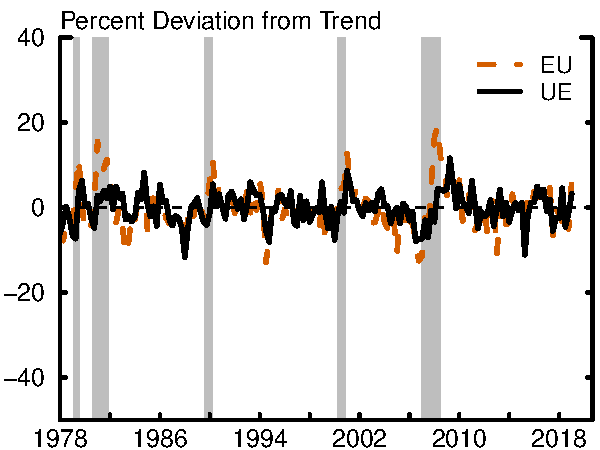
\includegraphics[scale=0.75]{grossflows_cyclicality_hpf.pdf}
\end{subfigure}
\vspace{0.5cm}
\begin{adjustwidth}{0.75cm}{0.75cm}
\footnotesize Notes: Black, solid lines show $U$-to-$E$ flows. Orange, dashed lines show $E$-to-$U$ flows. Series HP-filtered with smoothing parameter 1,600. I take a quarterly average of monthly values before applying the filter. Monthly series are adjusted for seasonal variation and time aggregation bias.
\end{adjustwidth}
\end{figure}

\begin{figure}[H]
\centering
\caption{Cross-Correlations of Flow Probabilities (HP-Filtered)}\label{app:fig:crosscorr_flows_hpf}
\begin{subfigure}{.3275\textwidth}
\subcaption{$P_t(UE)$ and $P_{t + j}(EU)$}\label{app:fig:crosscorr_flows_a}\vspace{-0.25cm}
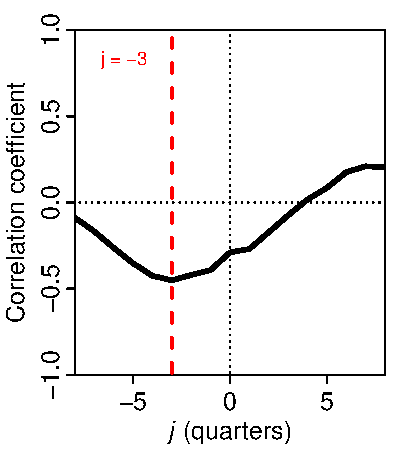
\includegraphics[scale=0.7]{flows_crosscorr_ue_eu_hpf.pdf}
\end{subfigure}
\begin{subfigure}{.3275\textwidth}
\subcaption{$u_t$ and $P_{t + j}(EU)$}\label{app:fig:crosscorr_flows_b}\vspace{-0.25cm}
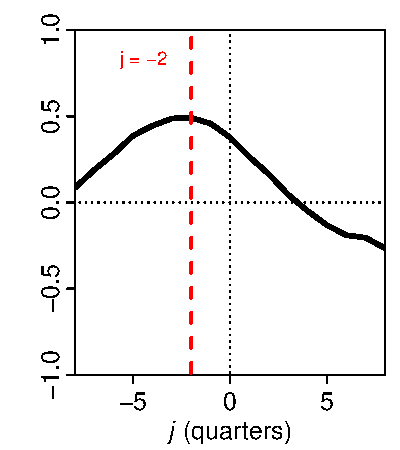
\includegraphics[scale=0.7]{flows_crosscorr_ur_eu_hpf.pdf}
\end{subfigure}
\begin{subfigure}{.3275\textwidth}
\subcaption{$u_t$ and $P_{t + j}(UE)$}\label{app:fig:crosscorr_flows_c}\vspace{-0.25cm}
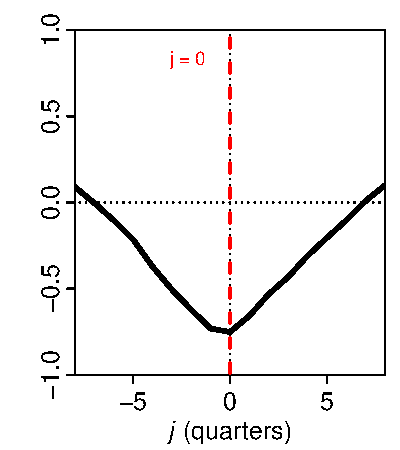
\includegraphics[scale=0.7]{flows_crosscorr_ur_ue_hpf.pdf}
\end{subfigure}
\vspace{0.25cm}
\begin{adjustwidth}{0.75cm}{0.75cm}
\footnotesize Notes: Series HP-filtered with smoothing parameter 1,600. I take a quarterly average of monthly values before applying the filter. Monthly series are adjusted for seasonal variation and time aggregation bias. Correlation coefficient is the Kendall rank correlation coefficient. Sample = 1980Q4--2017Q4.  
\end{adjustwidth}
\end{figure}

\newpage
\subsection{Alternative Specifications}

This section contains robustness checks for the main empirical results. I consider three extensions of the main specification I estimate in Section \ref{sec:empirics}:
\begin{enumerate}
\item Increasing the lag length $p$ from 4 to 8 quarters
\item Including 2020Q1--2024Q4 in the sample to assess the effects of the pandemic
\item Including additional macroeconomic variables -- GDP and vacancies -- in the VAR
\end{enumerate}
The first two extensions are straightforward. For the last, including two additional variables in the VAR requires imposing additional restrictions on the impact matrix. I impose a recursive ordering scheme (zero restrictions) and order GDP last. I maintain the same restrictions on the joint behavior of the first four variables in the VAR as in the main text. Across all robustness specifications considered, I obtain broadly consistent estimates as in my main specification.

\newpage
\subsubsection{Increasing Lag Length ($p = 8$)}
\begin{figure}[H]
\centering
\caption{Response to Unemployment Inflow Shock}
\begin{subfigure}{.24\textwidth}
\centering
\subcaption{Job Separation}\vspace{-0.1cm}
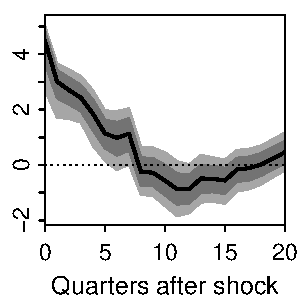
\includegraphics[scale=0.75]{robustness/lags/zerosign_ir_v1_e1.pdf}
\end{subfigure}
\begin{subfigure}{.24\textwidth}
\centering
\subcaption{Job Finding}\vspace{-0.1cm}
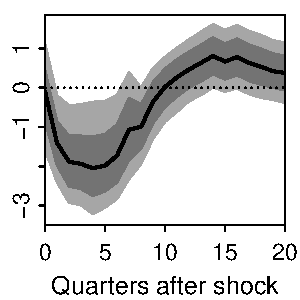
\includegraphics[scale=0.75]{robustness/lags/zerosign_ir_v2_e1.pdf}
\end{subfigure}
\begin{subfigure}{.24\textwidth}
\centering
\subcaption{Unemployment}\vspace{-0.1cm}
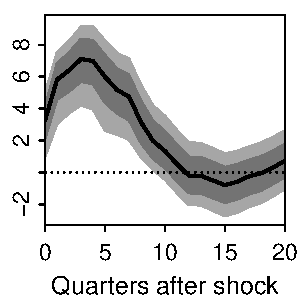
\includegraphics[scale=0.75]{robustness/lags/zerosign_ir_v3_e1.pdf}
\end{subfigure}
\begin{subfigure}{.24\textwidth}
\centering
\subcaption{Average Duration}\vspace{-0.1cm}
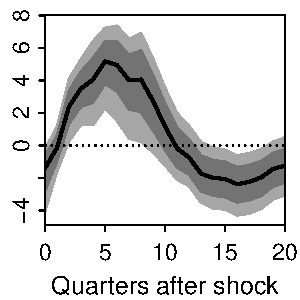
\includegraphics[scale=0.75]{robustness/lags/zerosign_ir_v4_e1.pdf}
\end{subfigure}
\end{figure}

\begin{figure}[H]
\centering
\caption{Response to Unemployment Outflow Shock}
\begin{subfigure}{.24\textwidth}
\centering
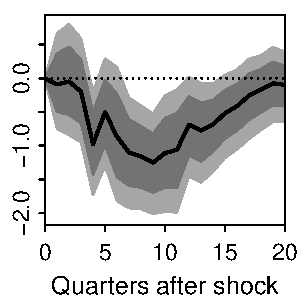
\includegraphics[scale=0.75]{robustness/lags/zerosign_ir_v1_e2.pdf}
\end{subfigure}
\begin{subfigure}{.24\textwidth}
\centering
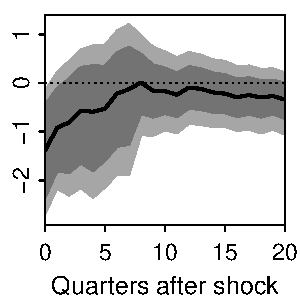
\includegraphics[scale=0.75]{robustness/lags/zerosign_ir_v2_e2.pdf}
\end{subfigure}
\begin{subfigure}{.24\textwidth}
\centering
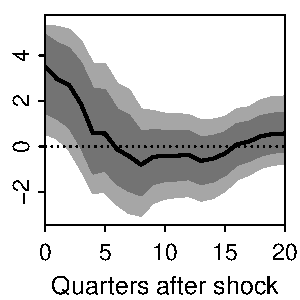
\includegraphics[scale=0.75]{robustness/lags/zerosign_ir_v3_e2.pdf}
\end{subfigure}
\begin{subfigure}{.24\textwidth}
\centering
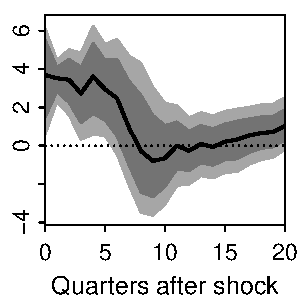
\includegraphics[scale=0.75]{robustness/lags/zerosign_ir_v4_e2.pdf}
\end{subfigure}
\end{figure}

\begin{figure}[H]
\centering
\caption{Response to Unemployment Level Shock}
\begin{subfigure}{.24\textwidth}
\centering
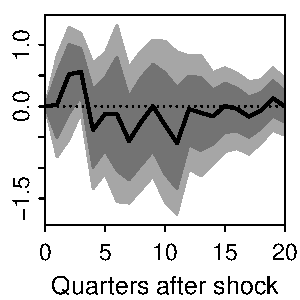
\includegraphics[scale=0.75]{robustness/lags/zerosign_ir_v1_e3.pdf}
\end{subfigure}
\begin{subfigure}{.24\textwidth}
\centering
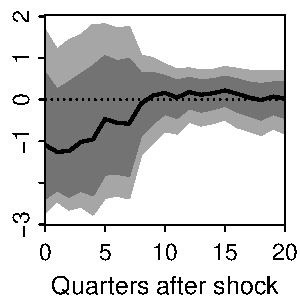
\includegraphics[scale=0.75]{robustness/lags/zerosign_ir_v2_e3.pdf}
\end{subfigure}
\begin{subfigure}{.24\textwidth}
\centering
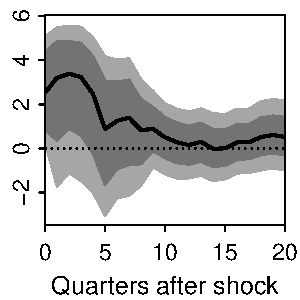
\includegraphics[scale=0.75]{robustness/lags/zerosign_ir_v3_e3.pdf}
\end{subfigure}
\begin{subfigure}{.24\textwidth}
\centering
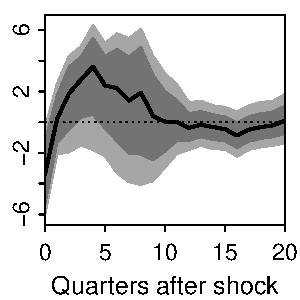
\includegraphics[scale=0.75]{robustness/lags/zerosign_ir_v4_e3.pdf}
\end{subfigure}
\end{figure}

\begin{figure}[H]
\centering
\caption{Response to Unemployment Length Shock}
\begin{subfigure}{.24\textwidth}
\centering
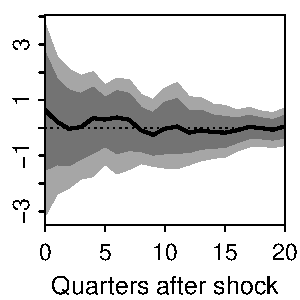
\includegraphics[scale=0.75]{robustness/lags/zerosign_ir_v1_e4.pdf}
\end{subfigure}
\begin{subfigure}{.24\textwidth}
\centering
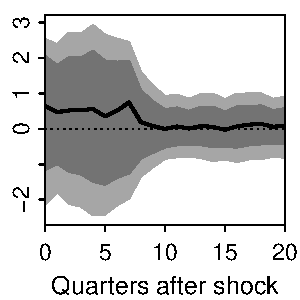
\includegraphics[scale=0.75]{robustness/lags/zerosign_ir_v2_e4.pdf}
\end{subfigure}
\begin{subfigure}{.24\textwidth}
\centering
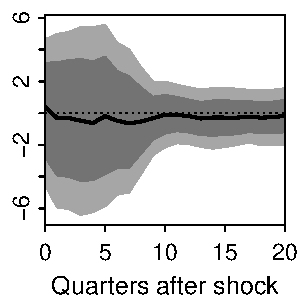
\includegraphics[scale=0.75]{robustness/lags/zerosign_ir_v3_e4.pdf}
\end{subfigure}
\begin{subfigure}{.24\textwidth}
\centering
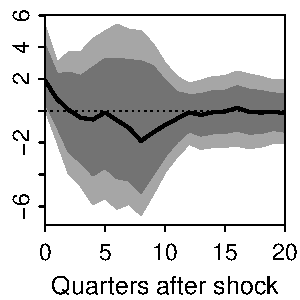
\includegraphics[scale=0.75]{robustness/lags/zerosign_ir_v4_e4.pdf}
\end{subfigure}
\end{figure}

\newpage
\subsubsection{Extending Sample}
\begin{figure}[H]
\centering
\caption{Response to Unemployment Inflow Shock}
\begin{subfigure}{.24\textwidth}
\centering
\subcaption{Job Separation}\vspace{-0.1cm}

\includegraphics[scale=0.75]{robustness/sample/zerosign_ir_v1_e1.pdf}
\end{subfigure}
\begin{subfigure}{.24\textwidth}
\centering
\subcaption{Job Finding}\vspace{-0.1cm}

\includegraphics[scale=0.75]{robustness/sample/zerosign_ir_v2_e1.pdf}
\end{subfigure}
\begin{subfigure}{.24\textwidth}
\centering
\subcaption{Unemployment}\vspace{-0.1cm}

\includegraphics[scale=0.75]{robustness/sample/zerosign_ir_v3_e1.pdf}
\end{subfigure}
\begin{subfigure}{.24\textwidth}
\centering
\subcaption{Average Duration}\vspace{-0.1cm}

\includegraphics[scale=0.75]{robustness/sample/zerosign_ir_v4_e1.pdf}
\end{subfigure}
\end{figure}

\begin{figure}[H]
\centering
\caption{Response to Unemployment Outflow Shock}
\begin{subfigure}{.24\textwidth}
\centering

\includegraphics[scale=0.75]{robustness/sample/zerosign_ir_v1_e2.pdf}
\end{subfigure}
\begin{subfigure}{.24\textwidth}
\centering

\includegraphics[scale=0.75]{robustness/sample/zerosign_ir_v2_e2.pdf}
\end{subfigure}
\begin{subfigure}{.24\textwidth}
\centering

\includegraphics[scale=0.75]{robustness/sample/zerosign_ir_v3_e2.pdf}
\end{subfigure}
\begin{subfigure}{.24\textwidth}
\centering

\includegraphics[scale=0.75]{robustness/sample/zerosign_ir_v4_e2.pdf}
\end{subfigure}
\end{figure}

\begin{figure}[H]
\centering
\caption{Response to Unemployment Level Shock}
\begin{subfigure}{.24\textwidth}
\centering

\includegraphics[scale=0.75]{robustness/sample/zerosign_ir_v1_e3.pdf}
\end{subfigure}
\begin{subfigure}{.24\textwidth}
\centering

\includegraphics[scale=0.75]{robustness/sample/zerosign_ir_v2_e3.pdf}
\end{subfigure}
\begin{subfigure}{.24\textwidth}
\centering

\includegraphics[scale=0.75]{robustness/sample/zerosign_ir_v3_e3.pdf}
\end{subfigure}
\begin{subfigure}{.24\textwidth}
\centering

\includegraphics[scale=0.75]{robustness/sample/zerosign_ir_v4_e3.pdf}
\end{subfigure}
\end{figure}

\begin{figure}[H]
\centering
\caption{Response to Unemployment Length Shock}
\begin{subfigure}{.24\textwidth}
\centering

\includegraphics[scale=0.75]{robustness/sample/zerosign_ir_v1_e4.pdf}
\end{subfigure}
\begin{subfigure}{.24\textwidth}
\centering

\includegraphics[scale=0.75]{robustness/sample/zerosign_ir_v2_e4.pdf}
\end{subfigure}
\begin{subfigure}{.24\textwidth}
\centering

\includegraphics[scale=0.75]{robustness/sample/zerosign_ir_v3_e4.pdf}
\end{subfigure}
\begin{subfigure}{.24\textwidth}
\centering

\includegraphics[scale=0.75]{robustness/sample/zerosign_ir_v4_e4.pdf}
\end{subfigure}
\end{figure}

\newpage
\subsubsection{Including Additional Variables}
\begin{figure}[H]
\centering
\caption{Response to Unemployment Inflow Shock}
\begin{subfigure}{.24\textwidth}
\centering
\subcaption{Job Separation}\vspace{-0.1cm}

\includegraphics[scale=0.75]{robustness/specification/zerosign_ir_v1_e1.pdf}
\end{subfigure}
\begin{subfigure}{.24\textwidth}
\centering
\subcaption{Job Finding}\vspace{-0.1cm}

\includegraphics[scale=0.75]{robustness/specification/zerosign_ir_v2_e1.pdf}
\end{subfigure}
\begin{subfigure}{.24\textwidth}
\centering
\subcaption{Unemployment}\vspace{-0.1cm}

\includegraphics[scale=0.75]{robustness/specification/zerosign_ir_v3_e1.pdf}
\end{subfigure}
\begin{subfigure}{.24\textwidth}
\centering
\subcaption{Average Duration}\vspace{-0.1cm}

\includegraphics[scale=0.75]{robustness/specification/zerosign_ir_v4_e1.pdf}
\end{subfigure}
\end{figure}

\begin{figure}[H]
\centering
\caption{Response to Unemployment Outflow Shock}
\begin{subfigure}{.24\textwidth}
\centering

\includegraphics[scale=0.75]{robustness/specification/zerosign_ir_v1_e2.pdf}
\end{subfigure}
\begin{subfigure}{.24\textwidth}
\centering

\includegraphics[scale=0.75]{robustness/specification/zerosign_ir_v2_e2.pdf}
\end{subfigure}
\begin{subfigure}{.24\textwidth}
\centering

\includegraphics[scale=0.75]{robustness/specification/zerosign_ir_v3_e2.pdf}
\end{subfigure}
\begin{subfigure}{.24\textwidth}
\centering

\includegraphics[scale=0.75]{robustness/specification/zerosign_ir_v4_e2.pdf}
\end{subfigure}
\end{figure}

\begin{figure}[H]
\centering
\caption{Response to Unemployment Level Shock}
\begin{subfigure}{.24\textwidth}
\centering

\includegraphics[scale=0.75]{robustness/specification/zerosign_ir_v1_e3.pdf}
\end{subfigure}
\begin{subfigure}{.24\textwidth}
\centering

\includegraphics[scale=0.75]{robustness/specification/zerosign_ir_v2_e3.pdf}
\end{subfigure}
\begin{subfigure}{.24\textwidth}
\centering

\includegraphics[scale=0.75]{robustness/specification/zerosign_ir_v3_e3.pdf}
\end{subfigure}
\begin{subfigure}{.24\textwidth}
\centering

\includegraphics[scale=0.75]{robustness/specification/zerosign_ir_v4_e3.pdf}
\end{subfigure}
\end{figure}

\begin{figure}[H]
\centering
\caption{Response to Unemployment Length Shock}
\begin{subfigure}{.24\textwidth}
\centering

\includegraphics[scale=0.75]{robustness/specification/zerosign_ir_v1_e4.pdf}
\end{subfigure}
\begin{subfigure}{.24\textwidth}
\centering

\includegraphics[scale=0.75]{robustness/specification/zerosign_ir_v2_e4.pdf}
\end{subfigure}
\begin{subfigure}{.24\textwidth}
\centering

\includegraphics[scale=0.75]{robustness/specification/zerosign_ir_v3_e4.pdf}
\end{subfigure}
\begin{subfigure}{.24\textwidth}
\centering

\includegraphics[scale=0.75]{robustness/specification/zerosign_ir_v4_e4.pdf}
\end{subfigure}
\end{figure}

\begin{figure}[H]
\centering
\caption{Response to Vacancy Shock}
\begin{subfigure}{.24\textwidth}
\centering
\subcaption{Job Separation}\vspace{-0.1cm}
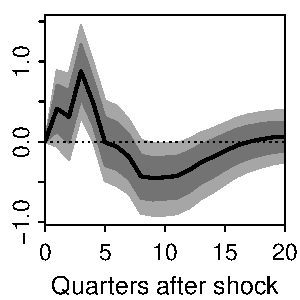
\includegraphics[scale=0.75]{robustness/specification/zerosign_ir_v1_e5.pdf}
\end{subfigure}
\begin{subfigure}{.24\textwidth}
\centering
\subcaption{Job Finding}\vspace{-0.1cm}
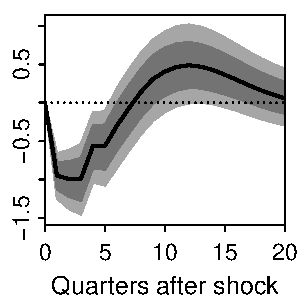
\includegraphics[scale=0.75]{robustness/specification/zerosign_ir_v2_e5.pdf}
\end{subfigure}
\begin{subfigure}{.24\textwidth}
\centering
\subcaption{Unemployment}\vspace{-0.1cm}
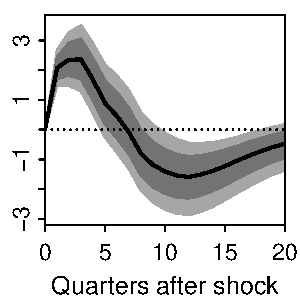
\includegraphics[scale=0.75]{robustness/specification/zerosign_ir_v3_e5.pdf}
\end{subfigure}
\begin{subfigure}{.24\textwidth}
\centering
\subcaption{Average Duration}\vspace{-0.1cm}
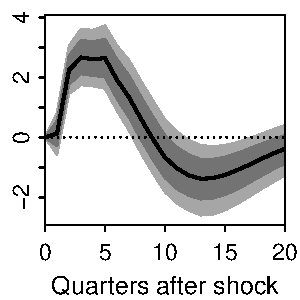
\includegraphics[scale=0.75]{robustness/specification/zerosign_ir_v4_e5.pdf}
\end{subfigure}
\end{figure}

\begin{figure}[H]
\centering
\caption{Response to GDP Shock}
\begin{subfigure}{.24\textwidth}
\centering
\subcaption{Job Separation}\vspace{-0.1cm}
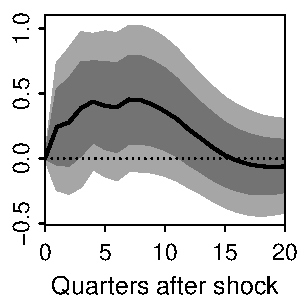
\includegraphics[scale=0.75]{robustness/specification/zerosign_ir_v1_e6.pdf}
\end{subfigure}
\begin{subfigure}{.24\textwidth}
\centering
\subcaption{Job Finding}\vspace{-0.1cm}
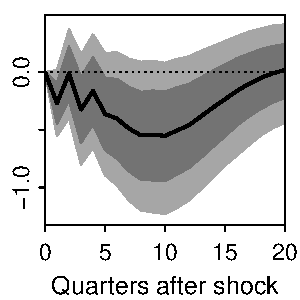
\includegraphics[scale=0.75]{robustness/specification/zerosign_ir_v2_e6.pdf}
\end{subfigure}
\begin{subfigure}{.24\textwidth}
\centering
\subcaption{Unemployment}\vspace{-0.1cm}
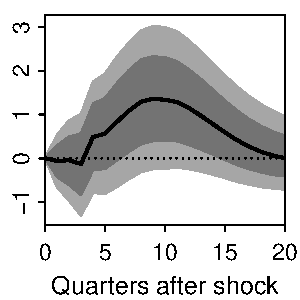
\includegraphics[scale=0.75]{robustness/specification/zerosign_ir_v3_e6.pdf}
\end{subfigure}
\begin{subfigure}{.24\textwidth}
\centering
\subcaption{Average Duration}\vspace{-0.1cm}
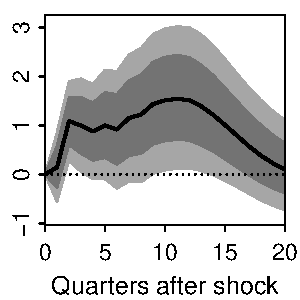
\includegraphics[scale=0.75]{robustness/specification/zerosign_ir_v4_e6.pdf}
\end{subfigure}
\end{figure}

\begin{figure}[H]
\centering
\caption{Response of Vacancies and GDP to Inflow and Outflow Shocks}
\begin{subfigure}{.24\textwidth}
\centering
\subcaption{Vacancies: Inflow}\vspace{-0.1cm}
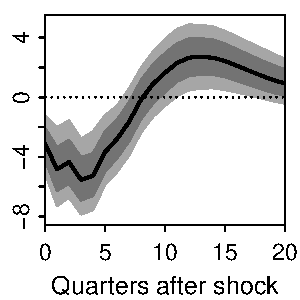
\includegraphics[scale=0.75]{robustness/specification/zerosign_ir_v5_e1.pdf}
\end{subfigure}
\begin{subfigure}{.24\textwidth}
\centering
\subcaption{Vacancies: Outflow}\vspace{-0.1cm}
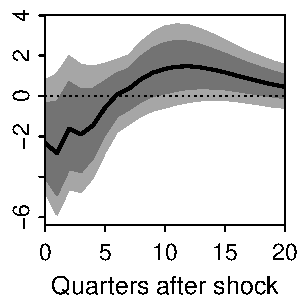
\includegraphics[scale=0.75]{robustness/specification/zerosign_ir_v5_e2.pdf}
\end{subfigure}
\begin{subfigure}{.24\textwidth}
\centering
\subcaption{GDP: Inflow}\vspace{-0.1cm}
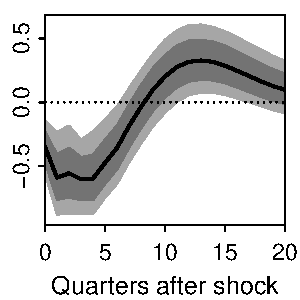
\includegraphics[scale=0.75]{robustness/specification/zerosign_ir_v6_e1.pdf}
\end{subfigure}
\begin{subfigure}{.24\textwidth}
\centering
\subcaption{GDP: Outflow}\vspace{-0.1cm}
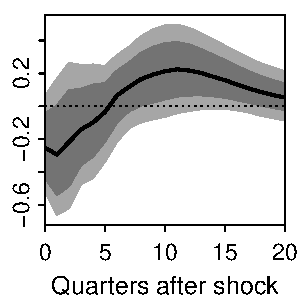
\includegraphics[scale=0.75]{robustness/specification/zerosign_ir_v6_e2.pdf}
\end{subfigure}
\end{figure}

\newpage
\section{Derivations and Proofs}\label{app:sec:proofs}

This appendix contains additional detail on the decompositions I perform in Section \ref{sec:results} of the paper. Below, I show how to compute the shock contribution to the variance of the endogenous variables in closed form. I also provide the formulas I use to construct the forecast error variance decomposition and historical decomposition. 

\subsection{Closed-Form Solution for Variance of VAR$(p)$}

Let the vector autoregression (VAR) model of order $p$ be given by the equation below.\footnote{Note that the notation used to define the VAR is slightly different than in the main text.}
\begin{equation}\label{app:eqn:varp_model}
Y_{t} = B_0 + B_1 Y_{t-1} + B_2 Y_{t-2} + \dots + B_p Y_{t-p} + U_t
\end{equation}
Let $n$ be the number of variables in the model. In the equation above, $Y_t$ is a $n \times 1$ column vector of endogenous variables, $U_t$ is a $n \times 1$ column vector of (reduced-form) residuals, $B_0$ is a $n \times 1$ column vector of intercept terms, and $B_1, \dots, B_p$ are $n \times n$ matrices of coefficients.

\paragraph{Companion Form} First, we transform the VAR$(p)$ model above into a VAR$(1)$ model by constructing its companion form. Let the variance-covariance matrix of the residuals $U_t$ be given by $\Var (U_t) = \Sigma$. Let $\mathbf{Y}_{t}$ denote the $np \times 1$ \textit{stacked} column vector of endogenous variables and let $\mathbf{U}_{t}$ denote the $np \times 1$ \textit{stacked} column vector of residuals. Let $\mathbf{B}_0$ denote the $np \times 1$ \textit{stacked} column vector of intercept terms and $\mathbf{B}_1$ denote the $np \times np$ matrix of coefficients. These objects and their relationship to Equation (\ref{app:eqn:varp_model}) are given below.
$$
\underbrace{\begin{bmatrix}
Y_{t} \\
Y_{t-1} \\
\vdots \\
Y_{t-p}
\end{bmatrix}}_{\mathbf{Y}_{t}}
= 
\underbrace{\begin{bmatrix}
B_0 \\
0 \\
\vdots \\
0
\end{bmatrix}}_{\mathbf{B}_0}
+
\underbrace{\begin{bmatrix}
B_1 & B_2 & \dots & B_p \\
I_n & 0 & \dots & 0 \\
\vdots & \ddots & \ddots & \vdots \\
0 & \dots & I_n & 0 \\
\end{bmatrix}}_{\mathbf{B}_1}
\underbrace{\begin{bmatrix}
Y_{t-1} \\
Y_{t-2} \\
\vdots \\
Y_{t-p-1}
\end{bmatrix}}_{\mathbf{Y}_{t-1}}
+
\underbrace{\begin{bmatrix}
U_{t} \\
0 \\
\vdots \\
0
\end{bmatrix}}_{\mathbf{U}_{t}}
$$
Note that the first row of this relation simply restates Equation (\ref{app:eqn:varp_model}). Each subsequent row states that $\mathbf{Y}_{t-j} = \mathbf{Y}_{t-j}$ for $j = 1,\dots,p$. Therefore, the companion form is given by 
\begin{equation}\label{app:eqn:companion_form}
\mathbf{Y}_t = \mathbf{B}_0 + \mathbf{B}_1 \mathbf{Y}_{t-1} + \mathbf{U}_t 
\end{equation}
Notice that this is a VAR model of order 1.

\paragraph{Variance Matrix of Endogenous Variables}

Define the following expression for the variance of the vector of endogenous variables.
$$ \mathbf{\Gamma} \equiv \Var(\mathbf{Y}_t) = 
\begin{bmatrix}
\Var(Y_t) & \Cov(Y_t, Y_{t-1}) & \dots & \Cov(Y_t, Y_{t-p}) \\
\Cov(Y_{t-1},Y_t) & \Var(Y_{t-1}) & \dots & \Cov(Y_{t-1}, Y_{t-p}) \\
\vdots & \ddots & \ddots & \vdots \\
\Cov(Y_{t-p},Y_t) & \dots & \dots & \Var(Y_{t-p}) \\
\end{bmatrix}$$
The matrix $\mathbf{\Gamma}$ is a $np \times np$ variance-covariance matrix whose entries $\Cov(Y_{t-i}, Y_{t-j})$ are themselves $n \times n$ variance-covariance matrices. Notice that the diagonal elements of $\mathbf{\Gamma}$ (i.e. where $i = j$) are simply the variance of the vector $Y_t$. When working with a (covariance-) stationary model, $\Var(Y_t) = \Var(Y_{t-1}) = \dots = \Var(Y_{t-p})$ in population. The off-diagonal elements are simply equal to the covariance of $Y_t$ with lags of itself. Hence, $\mathbf{\Gamma}$ has the familiar symmetry property of variance-covariance matrices. 

\paragraph{Variance Matrix of Residuals}

Define the following expression for the variance of the vector of residuals.
$$ \mathbf{\Omega} \equiv \Var(\mathbf{U}_t) = 
\begin{bmatrix}
\Var(U_t) & \dots & 0 \\
0 & \dots & 0 \\
\vdots & \ddots & \vdots \\
0 & \dots &0 \\
\end{bmatrix}
=
\begin{bmatrix}
\Sigma & \dots & 0 \\
0 & \dots & 0 \\
\vdots & \ddots & \vdots \\
0 & \dots &0 \\
\end{bmatrix}$$
The matrix $\mathbf{\Omega}$ is a $np \times np$ variance-covariance matrix where the first element is simply the variance of $Y_t$. All other elements are zero because of the definition of $\mathbf{U_t}$.

\begin{definition}
The variance of the endogenous variables in the VAR$(p)$ model is related to (i) the VAR coefficients and (ii) the variance of the residuals through the formula:
\begin{equation}\label{app:eqn:var_closed_form}
\vect(\mathbf{\Gamma}) = \left(\mathbb{I}_{M}  - \mathbf{B_1} \otimes \mathbf{B_1}\right)^{-1} \vect(\mathbf{\Omega})
\end{equation}
where $M = (np)^2 \times (np)^2$, $\otimes$ is the Kronecker product, and $(\cdot)^{-1}$ represents the matrix inverse.\footnote{See \cite{Hamilton:1994aa} Chapter 10.2, pages 265-266 for a similar derivation.}
\begin{proof}
Start with the definition of $\mathbf{\Gamma} = \Var(\mathbf{Y}_t)$. Then, plug in the expression for the companion form in Equation (\ref{app:eqn:companion_form}) and reduce.
\begin{align*}
\mathbf{\Gamma} = & \ \Var(\mathbf{Y}_t) \\
= & \ \Var(\mathbf{B}_0 + \mathbf{B}_1 \mathbf{Y}_{t-1} + \mathbf{U}_t) \\
= & \ \Var(\mathbf{B}_0) + \Var(\mathbf{B}_1 \mathbf{Y}_{t-1}) + \Var(\mathbf{U}_t) \\
= & \ 0 + \mathbf{B}_1\underbrace{\Var(\mathbf{Y}_{t-1})}_{\mathbf{\Gamma}}\mathbf{B}_1^\prime + \mathbf{\Omega}
\end{align*}
We have that $\mathbf{\Gamma} =  \mathbf{B}_1\mathbf{\Gamma}\mathbf{B}_1^\prime + \mathbf{\Omega}$. To solve for $\mathbf{\Gamma}$, we make use of the ``vec'' operator $\vect(\cdot)$.
\begin{align*}
\vect(\mathbf{\Gamma}) = & \ \vect(\mathbf{B}_1\mathbf{\Gamma}\mathbf{B}_1^\prime + \mathbf{\Omega}) \\
= & \ \vect(\mathbf{B}_1\mathbf{\Gamma}\mathbf{B}_1^\prime) + \vect(\mathbf{\Omega}) \\
= & \ (\mathbf{B}_1 \otimes \mathbf{B}_1)\vect(\mathbf{\Gamma}) + \vect(\mathbf{\Omega}) \\
\end{align*}
Solving for $\vect(\mathbf{\Gamma})$ in the final line yields the desired result in Equation (\ref{app:eqn:var_closed_form}).
\end{proof}
\end{definition}

\paragraph{Estimation of Closed-Form Variance}

We can now make use of the above result contained in Equation (\ref{app:eqn:var_closed_form}) to compute the sample variance of a VAR$(p)$ model in closed form. The algorithm for doing so is as follows:
\begin{enumerate}
\item Estimate the VAR$(p)$ model given by Equation (\ref{app:eqn:varp_model}).
\item Obtain the estimated coefficients $\hat B_1, \dots, \hat B_p$ and estimated variance-covariance matrix of the residuals $\hat \Sigma$.
\item Construct the companion form coefficient matrix $\hat{\mathbf{B}}_1$ and companion form variance-covariance matrix of the residuals $\hat{\mathbf{\Omega}}$.
\item Compute $\vect(\hat{\mathbf{\Gamma}})$ using $\hat{\mathbf{B}}_1$, $\hat{\mathbf{\Omega}}$, and Equation (\ref{app:eqn:var_closed_form}). Then compute $\hat{\mathbf{\Gamma}} = \vect^{-1}(\vect(\hat{\mathbf{\Gamma}}))$.
\item The variance-covariance matrix of $Y_t$ is the first $n$ rows and $n$ columns of $\hat{\mathbf{\Gamma}}$.
\end{enumerate}
Therefore, we can find a closed-form estimate of the variance of the VAR$(p)$ model by first constructing $\hat{\mathbf{\Gamma}}$, and then taking the appropriate rows and columns.
\begin{equation}
\hat{\Gamma}_0 \equiv \hat{\Var}(Y_t) = \hat{\mathbf{\Gamma}}_{(1:n, 1:n)}
\end{equation}

\paragraph{Computing Conditional Variance}

We can use the relationship above to compute the variance of the endogenous variables \textit{conditional} on a given structural shock. Notice that because $U_t = A E_t$, 
$$\Sigma \equiv \Var(U_t) = \Var(A E_t) = A\underbrace{\Var(E_t)}_{\mathbb{I}_n}A^\prime = AA^\prime $$
Hence, once we have such a matrix $A$, we can replace $\Sigma$ with $AA^\prime$ in the formulas above to compute the variance of $Y_t$. To compute the variance of $Y_t$ conditional on some structural shock, we can follow the following procedure:
\begin{enumerate}
\item Obtain $A$ using one of the identification procedures discussed below.
\item To compute the variance conditional on the $j_{th}$ structural shock, construct $A_j = A\mathbf{e}_j$, where $\mathbf{e}_j = [0,\dots,0,1,0,\dots,0]^\prime$ is the column-wise basis vector, with 1 in the $j_{th}$ row and 0 elsewhere. 
\item Replace $\Sigma$ with $A_jA_j^\prime$ in the formulas above.
\end{enumerate}

Let $\Var(Y_t | e_j)$ denote the variance of the endogenous variables conditional on the $j_{th}$ structural shock (i.e. where we have constructed $\mathbf{\Omega}$ using $A_jA_j^\prime$ instead of $\Sigma$). Because variance is additive and the structural shocks are independent, we have that
$$ \Var(Y_t) = \sum_j \Var(Y_t | e_j) $$
For VAR models estimated with sign restrictions, we set $A = CQ$, where $Q$ is an orthogonal matrix that satisfies the sign restriction and $C$ is the Cholesky decomposition of $\Sigma$.

\subsection{Formulas for Decompositions}

\paragraph{Forecast Error Variance Decomposition (FEVD)}

Let $\bar \phi_{i,j,h}$ be the median impulse response function of variable $i$ to shock $j$ at horizon $h$. $\bar \phi_{i,j,h}$ is obtained by computing the impulse response function for each $(i,j,h)$ and each draw $d$, and taking the pointwise median across draws. Then, the FEVD is given by the formula below.
\begin{equation}\label{app:eqn:fevd}
FEVD_{i,j,h} = \frac{\sum_{a = 1}^h (\bar \phi_{i,j,a})^2}{\sum_j \sum_{a = 1}^h (\bar \phi_{i,j,a})^2}
\end{equation} 

\paragraph{Historical Decomposition (HD)} The historical decomposition allows one to analyze the counterfactual evolution of each endogenous variable if only certain shocks had hit the economy during the sample period. Let $(B_l, \Sigma, Q)_d$ denote a draw of  the reduced form coefficients $B_l$, the variance-covariance matrix of the residuals $\Sigma$, and an orthogonal rotation matrix $Q$ that maps the structural shocks into the reduced form residuals. Let $\hat \mu_{t,d}$ denote the vector of reduced form residuals associated with this draw and let $\hat \varepsilon_{t,d} = A_d^{-1}\hat \mu_{t,d}$ denote the vector of structural shocks associated with this draw, where $A_d = C_d Q_d$ is the impact matrix and $C_d$ is the Cholesky decomposition of $\Sigma_d$. Now, iterate to form
$$ y_{t,j,d} = b_{0,d} + \sum_{l = 1}^L B_{l,d} y_{t-l,j,d} + \hat \varepsilon_{t,d} A_d \mathbf{e}_j $$
for each time period $t$ in the sample period, where $\mathbf{e}_j$ is the $j_{th}$ basis vector, starting from an initial condition of $y_{0,j,d} = [0, \dots, 0]^\prime$. The pointwise median of $ y_{t,j,d}$ across draws $d$ is the evolution of $y_t$ under only shock $j$. Plotting $y_{t,j}$ across time for all shocks $j = 1, \dots, n$ shows the HD.

\paragraph{Local Projections (LPs)}

To compute local projections, I employ a similar strategy. As above, let $(B_l, \Sigma, Q)_d$ denote a draw of  the reduced form coefficients $B_l$, the variance-covariance matrix of the residuals $\Sigma$, and an orthogonal rotation matrix $Q$ that maps the structural shocks into the reduced form residuals. Let $\hat \mu_{t,d}$ denote the vector of reduced form residuals associated with this draw and let $\hat \varepsilon_{t,d} = A_d^{-1}\hat \mu_{t,d}$ denote the vector of structural shocks associated with this draw, where $A_d = C_d Q_d$ is the impact matrix and $C_d$ is the Cholesky decomposition of $\Sigma_d$.

For each draw $d$, variable $i$, shock $j$, and horizon $h$, I estimate
$$ y_{t+h,i,j,d} = \alpha^h_{i,j,d} + \beta^h_{i,j,d}\,\hat \varepsilon_{t,j,d} + u_{t+h,i,j,d} \text{.} $$
The coefficient $\beta^h_{i,j,d}$ represents the impulse response of variable $i$ at horizon $h$ to shock $j$ for draw $d$. I also obtain the associated confidence intervals of $\beta^h_{i,j,d}$. I then plot the pointwise median across draws of the point estimates and confidence intervals.

\end{document}
